%% RiSE Latex Template - version 0.5
%%
%% RiSE's latex template for thesis and dissertations
%% http://risetemplate.sourceforge.net
%%
%% (c) 2012 Yguaratã Cerqueira Cavalcanti (yguarata@gmail.com)
%%          Vinicius Cardoso Garcia (vcg@cin.ufpe.br)
%%
%% This document was initially based on UFPEThesis template, from Paulo Gustavo
%% S. Fonseca.
%%
%% ACKNOWLEDGEMENTS
%%
%% We would like to thanks the RiSE's researchers community, the 
%% students from Federal University of Pernambuco, and other users that have
%% been contributing to this projects with comments and patches.
%%
%% GENERAL INSTRUCTIONS
%%
%% We strongly recommend you to compile your documents using pdflatex command.
%% It is also recommend use the texlipse plugin for Eclipse to edit your documents.
%%
%% Options for \documentclass command:
%%         * Idiom
%%           pt   - Portguese (default)
%%           en   - English
%%
%%         * Text type
%%           bsc  - B.Sc. Thesis
%%           msc  - M.Sc. Thesis (default)
%%           qual - PHD qualification (not tested yet)
%%           prop - PHD proposal (not tested yet)
%%           phd  - PHD thesis
%%
%%         * Media
%%           scr  - to eletronic version (PDF) / see the users guide
%%
%%         * Pagination
%%           oneside - unique face press
%%           twoside - two faces press
%%
%%		   * Line spacing
%%           singlespacing  - the same as using \linespread{1}
%%           onehalfspacing - the same as using \linespread{1.3}
%%           doublespacing  - the same as using \linespread{1.6}
%%
%% Reference commands. Use the following commands to make references in your
%% text:
%%          \figref  -- for Figure reference
%%          \tabref  -- for Table reference
%%          \eqnref  -- for equation reference
%%          \chapref -- for chapter reference
%%          \secref  -- for section reference
%%          \appref  -- for appendix reference
%%          \axiref  -- for axiom reference
%%          \conjref -- for conjecture reference
%%          \defref  -- for definition reference
%%          \lemref  -- for lemma reference
%%          \theoref -- for theorem reference
%%          \corref  -- for corollary reference
%%          \propref -- for proprosition reference
%%          \pgref   -- for page reference
%%
%%          Example: See \chapref{chap:introduction}. It will produce 
%%                   'See Chapter 1', in case of English language.
%%
%% Citation commands:
%%          \citet (from natbib) -- To cite a reference as part of the narrative
%%          \citep (from natbib) -- To cite a reference between parenthesis
%%          citationblock environment -- To produce direct citation blocks according to the ABNT

\documentclass[pt,oneside,onehalfspacing,phd]{risethesis}

\usepackage{colortbl}
\usepackage{color}
\usepackage[table]{xcolor}
\usepackage{microtype}
\usepackage{bibentry}
\usepackage{subfigure}
\usepackage{multirow}
\usepackage{rotating}
\usepackage{booktabs}
\usepackage{pdfpages}
\usepackage{caption}
\usepackage{lipsum}
\usepackage{sectsty}
\usepackage{alltt}
\usepackage{pdfpages}

\captionsetup[table]{position=top,justification=centering,width=.85\textwidth,labelfont=bf,font=footnotesize}
\captionsetup[lstlisting]{position=top,justification=centering,width=.85\textwidth,labelfont=bf,font=footnotesize}
\captionsetup[figure]{position=bottom,justification=centering,width=.85\textwidth,labelfont=bf,font=footnotesize}

%% Chapter and (Sub)Section fonts must be same size as text (12)
\sectionfont{\fontsize{14}{15}\selectfont}
\subsectionfont{\fontsize{12}{15}\selectfont}
\subsubsectionfont{\fontsize{12}{15}\selectfont}

%% Change the following pdf author attribute name to your name.
\usepackage[linkcolor=black,
            citecolor=black,
            urlcolor=black,
            colorlinks,
            pdfpagelabels,
            pdftitle={Rise Thesis Template (ABNT)},
            pdfauthor={Rise Thesis Template (ABNT)},
            breaklinks=true]{hyperref}

\address{RECIFE}

\universitypt{Universidade Federal de Pernambuco}
\universityen{Federal University of Pernambuco}

\departmentpt{Centro de Informática}
\departmenten{Center for Informatics}

\programpt{Pós-graduação em Ciência da Computação}
\programen{Graduate in Computer Science}

\majorfieldpt{Ciência da Computação}
\majorfielden{Computer Science}

\title{ETL4NoSQL: Um framework de ETL para BDs NoSQL}

\date{2017}

\author{Carine Calixto Aguena}
\adviser{Valéria Cesário Times}
%\coadviser{Eduardo Santana de Almeida}

% Macros (defines your own macros here, if needed)
\def\x{\checkmark}

\begin{document}

\frontmatter

\frontpage

\presentationpage

\begin{fichacatalografica}
	\FakeFichaCatalografica % Comment this line when you have the correct file
%     \includepdf{fig_ficha_catalografica.pdf} % Uncomment this
\end{fichacatalografica}

\banca

\begin{dedicatory}
Eu dedico este trabalho à toda minha família, amigos e professores que me deram todo apoio necessário para alcançar meus objetivos.
\end{dedicatory}

\acknowledgements
\lipsum[1-4]

\begin{epigraph}[]{Osho}
Sempre que houver alternativas, tenha cuidado. Não opte pelo conveniente, pelo confortável, pelo respeitável, pelo socialmente aceitável, pelo honroso. 
Opte pelo que faz o seu coração vibrar. Opte pelo que gostaria de fazer, apesar de todas as consequências.
\end{epigraph}

\resumo
% Escreva seu resumo no arquivo resumo.tex
{\parindent0pt
	
Os procedimentos cruciais para a criação de \textit{data warehouses} e sistemas \acp{bi} são a integração de dados e os processos de ETL. Porém, os processo para ETL e integração de dados são comumente desenvolvidos para dados estruturados em modelos relacionais que representam apenas uma pequena parte dos dados mantidos por muitas empresas. Por isso, existe uma demanda crescente para integrar também os dados não estruturados e semi estruturados em um repositório unificado. Porém, devido a complexidade desses dados, novos desafios estão surgindo ao lidarmos com a heterogeneidade e distribuição dos dados em um ambiente de integração de dados.

Ademais, muitas empresas encontram dificuldades ao lidar com as ferramentas ETL disponíveis no mercado. Aprender a lidar com essas ferramentas pode ser muito custoso em termos financeiros e de tempo, e por isso, acabam optando desenvolver os seus processos por meio de uma linguagem de programação de propósito geral.

Portanto, propomos um \textit{framework} programável para desenvolvimento de sistemas de ETL que possibilita a integração de dados estruturados, não estruturados e semi estruturados armazenados em bases relacionais ou NoSQL, denominado ETL4NoSQL. Apresentamos os componentes do \textit{framework} ETL4NoSQL, bem como suas funcionalidades. Além disso, realizamos um estudo experimental de software, cujo teve como objetivo definir se o ETL4NoSQL é adequado para auxiliar no desenvolvimento de processos de ETL em dados estruturados, semi estruturados e não estruturados. Os resultados do estudo mostraram que o ETL4NoSQL possui um grau de similaridade de 70\% em relação com as outras 11 ferramentas estudadas nesta pesquisa, e que dessa similaridade 85,71\% das funcionalidades são consideradas úteis para desenvolver processos de ETL em dados estruturados, semi estruturados e não estruturados. 

Assim, podemos concluir que o objetivo da presente proposta, de especificar um \textit{framework} programável, flexível e integrado para extração, transformação e carga dos dados em BDs NoSQL foi atingido de forma efetiva e satisfatória, no sentido de facilitar e flexibilizar a atividade de desenvolvimento de novas ferramentas de ETL para dados estruturados, semi estruturados e não estruturados.

\begin{keywords}
ETL, Frameworks, NoSQL, Data Warehouse, Estudo Experimental de Software
\end{keywords}
}

\abstract
% Write your abstract in a file called abstract.tex
{\parindent0pt
	The crucial procedures for creating data warehouses and BI systems are data integration and ETL processes. However, processes for ETL and data integration are commonly developed for data structured in relational models that represent only a small part of the data maintained by many companies. Therefore, there is a growing demand to integrate both unstructured and semi-structured data into a unified repository. However, due to the complexity of these data, new challenges are emerging as we deal with the heterogeneity and distribution of data in the integration environment.

In addition, many companies encounter difficulties in dealing with the ETL tools available in the market. Learning how to handle these tools can be very costly in terms of time and financially, and so they end up opting to develop their processes through a general purpose programming language.

Therefore, we propose a programmable framework for the development of ETL systems that allows the integration of structured, unstructured and semi-structured data stored in relational bases or NoSQL, called ETL4NoSQL. We present the components of the ETL4NoSQL framework, as well as its functionalities. In addition, we conducted an experimental software study, whose purpose was to determine if ETL4NoSQL is adequate to assist in the development of ETL processes in structured, semi-structured and unstructured data. The results of the study showed that ETL4NoSQL has a degree of similarity of 70\% in relation to the other 11 tools studied in this research, and that of this similarity 85.71\% of the functionalities are considered useful to develop ETL processes in structured, semi structured and unstructured data.

Thus, we can conclude that the objective of the present proposal to specify a programmable, flexible and integrated framework for extracting, transforming and loading data into NoSQL BDs has been achieved in an effective and satisfactory way, in order to facilitate and make flexible the development activity of new ETL tools for structured, semi-structured and unstructured data.


\begin{keywords}
	ETL, Frameworks, NoSQL, Data Warehouse, Experimental Software Study
\end{keywords}

}

% List of figures
\listoffigures

% List of tables
\listoftables

% List of acronyms
% Acronyms manual: http://linorg.usp.br/CTAN/macros/latex/contrib/acronym/acronym.pdf
\listofacronyms
\begin{acronym}[ACRONYM] 
% Change the word ACRONYM above to change the acronym column width.
% The column width is equals to the width of the word that you put.
% Read the manual about acronym package for more examples:
%   http://linorg.usp.br/CTAN/macros/latex/contrib/acronym/acronym.pdf


\acro{apd}[APD]{Área de Processamento de Dado}
\acro{BDs NoSQL}[BDs NoSQL]{banco de dados NoSQL}
\acro{bi}[BI]{Business Intelligence}
\acro{dw}[DW]{Data Warehouse}
\acro{etl}[ETL]{Extract, Transform and Load}
\acro{rdbms}[RDBMS]{Relational Database Management System}
\acro{SGBD}[SGBD]{Sistema Gerenciador de Bancos de Dado}
\acro{OCL}{Object Constraint Language}


\acro{afm}[AFM]{Alphabet Frequency Matrix}
\acro{api}[API]{Application Programming Interface}
\acro{arima}[ARIMA]{Auto-Regressive Integrated Moving Average}
\acro{brn}[BRN]{Bug Report Network}
\acro{bts}[BTS]{Bug Triage System}
\acro{cas}[CAS]{Context-Aware Systems}
\acro{ccb}[CCB]{Change Control Board}
\acro{cr}[CR]{Change Request}
\acro{cvs}[CVS]{Concurrent Version System}
\acro{es}[ES]{Expert System}
\acro{floss}[FLOSS]{Free/Libre Open Source Software}
\acro{glr}[GLR]{Generalized Linear Regression}
\acro{gqm}[GQM]{Goal Question Metric}
\acro{html}[HTML]{HyperText Markup Language}
\acro{ir}[IR]{Information Retrieval}
\acro{irt}[IRT]{Recôncavo Institute of Technology}
\acro{jdt}[JDT]{Jazz Duplicate Finder}
\acro{lda}[LDA]{Latent Dirichlet Allocation}
\acro{loc}[LOC]{Lines of Code}
\acro{lsi}[LSI]{Latent Semantic Indexing}
\acro{ms}[MS]{Mapping Study}
\acro{msr}[MSR]{Mining Software Repositories}
\acro{nlp}[NLP]{Natural Language Processing}
\acro{promise}[PROMISE]{Predictive Models in Software Engineering}
\acro{rbes}[RBES]{Rule-Based Expert System}
\acro{rhel}[RHEL]{RedHat Enterprise Linux}
\acro{saas}[SaaS]{Software as a Service}
\acro{scm}[SCM]{Software Configuration Management}
\acro{serpro}[SERPRO]{Brazilian Federal Organization for Data Processing}
\acro{slr}[SLR]{Stepwise Linear Regression}
\acro{slr}[SLR]{Systematic Literature Review}
\acro{svd}[SVD]{Singular Value Decomposition}
\acro{svm}[SVM]{Support Vector Machine}
\acro{svn}[SVN]{Subversion}
\acro{tfidf}[TF-IDF]{Term Frequency-Inverse Document Frequency}
\acro{vsm}[VSM]{Vector Space Model}
\acro{xp}[XP]{Extreming Programming}
\end{acronym}

% Summary (tables of contents)
\tableofcontents

\mainmatter

\pagenumbering{arabic}

\chapter{Introdução}
\label{chp:introduction}

% \begin{quotation}[]{Poul Anderson}
% I have yet to see any problem, however complicated, which, when looked at in the
% right way, did not become still more complicated.
% \end{quotation}

\noindent Este capítulo contextualiza os principais assuntos abordados nesta dissertação, apresenta as motivações que levaram à escolha do tema, os objetivos gerais e específicos desta pesquisa, bem como a justificativa da investigação conduzida e suas principais contribuições.
\clearpage

% ----------------------------------------------------------
% seção
% ----------------------------------------------------------

\section{Contextualização}
% ----------------------------------------------------------

Desde a década de 1970, com a criação do modelo relacional por Edgar Frank Codd, a estrutura de armazenamento adotada por muitos desenvolvedores de sistemas da área de tecnologia da informação têm se baseado nesse conceito. A maioria dos sistemas gerenciadores de banco de dados (SGBD) que possui aceitação no mercado fazem uso desse modelo, por exemplo o MySQL, Oracle e Microsoft SQL Server. Porém, os requisitos de dados para o desenvolvimento de ferramentas de \textit{software} atual têm mudado significativamente, especialmente com o aumento das aplicações \textit{Web} (\cite{nasholm:2012}). Este segmento de aplicações exige alta escalabilidade e vazão, e SGBD relacionais muitas vezes não conseguem atender satisfatoriamente os seus requisitos de dados. Como alternativa a isso, novas abordagens de SGBD utilizando o termo de SGBD NoSQL tornaram-se popular (\cite{silva:2016}).

O termo NoSQL é constantemente interpretado como ''\emph{Not Only SQL}'' (não somente SQL), cujo SQL refere-se a linguagem disponibilizada pelos SGBD relacionais (\cite{nasholm:2012}). O propósito das abordagens NoSQL é oferecer alternativas onde os SGBD relacionais não apresentam um bom desempenho. Esse termo abrange diferentes tipos de sistemas. Em geral, SGBD NoSQL usam modelo de dados não-relacionais, com poucas definições de esquema, e geralmente, são executados em clusters. Alguns exemplos de SGBD NoSQL recentes são o Cassandra, MongoDB, Neo4J e o Riak (\cite{fowler:2013}).

Muitas empresas coletam e armazenam milhares de gigabytes de dados por dia, onde a análise desses dados representa uma vantagem competitiva no mercado. Por isso, há uma grande necessidade de novas arquiteturas para o suporte à decisão (\cite{liu:2013}). Para isso, uma das formas bastante utilizada é a criação de um ambiente \textit{data warehousing} responsável por providenciar informações estratégicas e esquematizadas a respeito do negócio (\cite{dayal:1997}).

Segundo a definição de \cite{kimball:2002}, \textit{data warehouse} (DW) é uma coleção de dados voltada para o processo de suporte à decisão, orientada por assunto, integrada, variante no tempo e não volátil. Os dados de diferentes fontes de dados são processados e integrados em um \textit{data warehouse} central através da Extração, Transformação e Carga (ETL) que é feita de maneira periódica. Os processos de ETL consistem em um conjunto de técnicas e ferramentas para transformar dados de múltiplas fontes de dados para fins de análise de negócio (\cite{silva:2016}). Ferramentas de ETL são sistemas de \textit{software} responsáveis por extrair dados de diversas fontes de dados, transformar, customizar e inseri-los no \textit{data warehouse}.

O projeto de ETL, ou seja, a criação dos seus processos, consome cerca de 70\% dos recursos de implantação de um DW, pois desenvolver esse projeto é crítico e custoso, tendo em vista que gerar dados incorretos pode acarretar em más decisões. Porém, por algum tempo pouca importância foi dada ao processo de ETL pelo fato de ser visto somente como uma atividade de suporte aos projetos de DW. Apenas a partir do ano 2000, a comunidade acadêmica passou a dar mais importância ao tema (\cite{silva:2012}). Atualmente, ainda existem dificuldades ao lidar com as soluções para ferramentas de ETL presentes na literatura. É comum que elas demonstrem mais importância aos SGBD relacionais. Pois, tradicionalmente o DW é implementado em um banco de dados relacional, onde o dado é armazenado nas tabelas fato e dimensões, que são descritas por um esquema em estrela (\cite{kimball:2002}). Por isso, para oferecer suporte aos sistemas que necessitem realizar os processos de ETL em banco de dados NoSQL, a proposta desse trabalho é especificar um \textit{framework} programável, flexível e integrado para modelagem e execução de processos de ETL em banco de dados NoSQL.

% ---
% Capitulo com exemplos de comandos inseridos de arquivo externo 
% ---
%\include{abntex2-modelo-include-comandos}
% ---

% ----------------------------------------------------------
% seção
% ----------------------------------------------------------
\section{Motivação}
% ----------------------------------------------------------

A integração de dados e os processos de ETL são procedimentos cruciais para a criação de \textit{data warehouses}. Porém, esses procedimentos são tradicionalmente desenvolvidos para dados em modelos relacionais, que representam apenas uma pequena parte dos dados mantidos por muitas empresas (\cite{darmont:2005}, \cite{russom:2007}, \cite{thomsen:2009}).

O uso generalizado da internet, web 2.0, redes sociais e sensores digitais produzem grandes volumes de dados. De fato, modelos de programação como o MapReduce (MR) introduzido pela Google (\cite{google:2004}), são executados continuamente para tratar mais de vinte Petabytes de dados por dia (\cite{dean:2008}). Esta explosão de dados é uma oportunidade para o surgimento de novas aplicações, como \textit{Big Data Analytics} (BDA); mas é, ao mesmo tempo, um problema dado as capacidades limitadas das máquinas e das aplicações tradicionais.

Esse grande volume de dados é conhecido como "\textit{Big Data}" e caracterizado pelos quatro "V": Volume, que implica a quantidade de dados que vão além das unidades de armazenamento usuais; a Velocidade com que esses dados são gerados e devem ser processados, a Variedade como diversidade de formatos e estruturas, e a Veracidade relacionada à precisão e confiabilidade dos dados. Assim, surgem novos paradigmas, tais como \textit{Cloud Computing} (Computação em Nuvem) e \textit{MapReduce} (MR), e novos modelos de dados são propostos para armazenamento de grandes volumes de dados, como o NoSQL (\textit{Not Only SQL}) (\cite{dean:2011}).

Dessa forma, existe uma demanda crescente para extrair, transformar e carregar grandes volumes de dados, apresentados de forma variada, em modelos não relacionais em um ambiente de suporte à decisão. Contudo, devido a complexidade desses dados, diferentes desafios estão surgindo quando lidamos com suas características, como por exemplo a heterogeneidade e distribuição desses dados, no ambiente de extração, transformação e carga de dados (\cite{salem:2012}).

Além disso, muitas empresas encontram dificuldades para lidar com as ferramentas de ETL disponíveis no mercado devido à sua longa curva de aprendizagem. Aprender a lidar com essas ferramentas pode ser muito custoso em termos financeiros e de tempo, e por isso, acabam optando desenvolver os seus processos por meio de uma linguagem de programação de propósito geral (\cite{awad:2011}, \cite{munoz:2009}).


%Uma maneira para organizar e manipular grandes volumes de dados sem utilizar um modelo relacional, e ainda processá-los e armazená-los de maneira distribuída é fazer o uso de BDs NoSQL (Bancos de Dados NoSQL) (\cite{scabora:2016}). Com isso, surge a necessidade de se promover meios para o uso desses bancos de dados em DWs. 

As pesquisas presentes na literatura sobre extração de dados em BDs NoSQL mostram que as ferramentas existentes no mercado propõem arquiteturas, metamodelos, aplicações e metodologias de modelagem para processos de ETL  ((\cite{silva:2016}, \cite{chevalier:2015}, \cite{liu:2013}).No entanto, elas não apresentam um framework programável em um ambiente integrado, e ainda ignoram conceitos importantes sobre frameworks, tais como reuso, flexibilidade, outros aspectos como a variedade dos dados e a falta de uma alternativa para substituir o SQL dos modelos relacionais.

Em geral, não é incomum observar que os especialistas em ETL utilizam interfaces textuais, enquanto que os não especialistas optem pelo uso de GUI. No entanto, mesmo que haja o envolvimento de membros não especializados em ETL, a implementação final dos processos é realizada por especialistas, os quais são mais eficientes quando utilizam interfaces de programação textuais (\cite{silva:2012}, \cite{mazanec:2012}).


Portanto, o aumento do uso de SGBD com modelos de dados não relacionais baseados no paradigma NoSQL e a falta de uma ferramenta programável, flexível e integrada, independente de plataforma que dê suporte à extração, transformação e carga para esses SGBD é a grande motivação deste trabalho.







% ----------------------------------------------------------
% Seção
% ----------------------------------------------------------
\section{Objetivos}

O objetivo principal desta pesquisa é especificar um \textit{framework} programável, flexível e integrado para modelagem e execução de processos de ETL de bancos de dados NoSQL. Baseamos nossa proposta nos princípios de flexibilidade, extensibilidade, reuso e inversão de controle, conforme recomenda a literatura sobre frameworks (\cite{awad:2011}, \cite{vassiliadis:2005}, \cite{fayad:1999}, \cite{fayad:1997}, \cite{darmont:2005}), além dos conceitos de desenvolvimento baseados em componentes apresentados na seção 2.1.3.

A arquitetura do ETL4NoSQL oferece uma interface de programação que contém elementos, tais como componentes de gerenciamento, leitura e escrita de dados, criação e execução de operações de ETL. O componente de gerenciamento é o responsável pelos fundamentos de ETL disponíveis na literatura (\cite{kimball:2004}). Ele possibilita as aplicações baseadas no ETL4NoSQL reutilizar os componentes para modelar seus processos de ETL. Além disso, a flexibilidade do framework proposto permite que sejam criados outros componentes que encapsulam regras de transformação para áreas especificas de ETL. Um componente especializado permite a construção de processos de ETL que não seriam possíveis ou que exigiriam o uso conjunto de muitos componentes genéricos do framework. Para possibilitar a criação de uma interface integrada para especialização e modelagem de processos de ETL, utilizamos o desenvolvimento baseado em componentes. Isto propiciou a implementação do ETL4NoSQL em uma linguagem de programação de propósito geral. Os objetivos específicos são detalhados a seguir.

\subsection{Objetivos Específicos}

Um dos objetivos específicos desta dissertação é apresentar a especificação e modelagem dos componentes do framework ETL4NoSQL, bem como suas interfaces e funcionalidades. Outro objetivo deste trabalho consiste em realizar um estudo experimental de \textit{software}, a fim de caracterizar as principais funcionalidades das ferramentas de ETL para BDs NoSQL. O estudo experimental tem como objetivo comparar o framework proposto neste trabalho e demonstrar suas vantagens e desvantagens em relação às ferramentas de ETL correlatas à este trabalho encontradas na literatura. Por fim, o nosso último objetivo é prover dois ambientes de ETL para facilitar a extração, transformação e carga de dados em DW modelados pelo esquema estrela, tendo em vista que este é o esquema de dados dimensional mais recomendado pela literatura (\cite{inmon:2002}, \cite{kimball:2002}). No primeiro ambiente utilizamos o SGBD MongoDB com dados sintéticos de ranking de restaurantes, e o segundo, o SGBD escolhido foi o CassandraDB com dados sintéticos de localizações de táxis.



%O primeiro objetivo específico desta pesquisa é estender a proposta do framework para facilitar a carga de dados de dois sistemas de BD NoSQL distintos baseado no mesmo paradigma NoSQL em um DW relacional modelados pelo esquema estrela, tendo em vista que este é o esquema de dados dimensionais mais recomendado pela literatura \cite{kimball:2002} \cite{Inmon: 2002}. O outro objetivo específico é ao invés de dar carga em um DW relacional fazer uso do mesmo sistema em um DW NoSQL, seguindo a metodologia adotada por \cite{chevalier:2015} em seu trabalho de pesquisa. Para isso, desenvolvemos dois frameworks especializados a partir do ETL4NoSQL em conformidade às peculiaridades dos processos de ETL nessas duas áreas de aplicação, os quais também são objetos de validação do ETL4NoSQL.

\section{Contribuições}

Uma das contribuições deste trabalho é o framework ETL4NoSQL. Ele permite extrair, transformar e carregar dados que estão armazenados em diversos SGBD NoSQL, ou até mesmo, repositórios de dados textuais e SGBD relacionais. A vantagem ao utilizar o ETL4NoSQL é sua natureza programável, flexível e integrada que facilita a modelagem e execução dos processos de ETL em banco de dados NoSQL.

Outra contribuição desta pesquisa é apresentar, por meio de um estudo experimental \textit{software} as principais funcionalidades de uma ferramenta de ETL, bem como possíveis melhorias, vantagens e desvantagens de acordo com os trabalhos correlatos encontrados na literatura.

Por fim, nossa última contribuição é oferecer duas aplicações de ETL, criadas a partir do ETL4NoSQL, utilizando domínios distintos baseados em dois sistemas NoSQL. 

\section{Organização do Trabalho}

Este trabalho está organizado de acordo com a seguinte estrutura:

\begin{itemize}
	\item \textbf{Fundamentação Teórica:} apresenta uma revisão de literatura sobre os principais assuntos abordados neste trabalho. São tratados temas a respeito de ETL, banco de dados NoSQL, frameworks, estudo experimental de \textit{software} e descreve os trabalhos correlatos encontrados na literatura a respeito de ferramentas de ETL.
	
	\item \textbf{O Framework ETL4NoSQL:} descreve os requisitos, a arquitetura de \textit{software} e implementação dos componentes do framework proposto.
			
	\item \textbf{Estudo Experimental de Software:} expõe o roteiro da experimentação de \textit{software} para ferramentas de ETL. Define o objetivo, o planejamento, a operação e o resultado do estudo.
	
	\item \textbf{Avaliação:} descreve aplicações de ETL4NoSQL para dois domínios de naturezas distintas, a fim de ilustrar a reusabilidade e flexibilidade do ETL4NoSQL, avaliando a proposta desta dissertação.
		
	\item \textbf{Considerações Finais:} expressa as limitações e ameaças à validade do trabalho, considerações finais e sugere de trabalhos futuros.	
	
\end{itemize}


\chapter{Fundamentação Teórica}

Neste capítulo, são apresentados os conceitos relacionados ao desenvolvimento desta pesquisa, bem como o embasamento teórico necessário para o entendimento do trabalho. Os assuntos abordados são: ETL, Banco de Dados NoSQL, \textit{Frameworks}, Estudo Experimental de \textit{Software} e trabalhos correlatos ao tema deste estudo.


\clearpage
% ---

\section{Conceitos Básicos}

Conceitos de ETL, banco de dados NoSQL, desenvolvimento baseado em componentes, \textit{frameworks} e estudo experimental de \textit{software} são essenciais para esta pesquisa. Dessa forma, os princípios básicos desses conceitos são apresentados nesta seção. Ainda que, estudo experimental de \textit{software} não seja o tema principal deste trabalho, seus conceitos são essenciais para avaliar e medir nossa proposta sendo fundamental entendê-los.

\subsection{ETL}

ETL (Extração, Limpeza/Transformação e Carga - ETL) é conhecido na literatura por definir processos que permitem a extração e transformação de dados, centralizando-os numa base destino facilitando o gerenciamento e análise desses dados (\cite{kimball:2004}, \cite{rud:2009}). O fluxo do processo de ETL inicia-se com extração dos dados a partir de uma fonte de dados, que podem ser arquivos textuais, banco de dados relacionais, banco de dados NoSQL, entre outros. Os dados são propagados para uma Área de Processamento de Dados (APD) onde são executadas a limpeza e transformação por meio de mecanismos de ETL definidos como agregação, junção, filtro, união, etc. Finalmente, os dados são carregados em estruturas que podem ser \textit{data warehouses} ou repositórios analíticos (\cite{silva:2016}, \cite{silva:2012}, \cite{kimball:2004}). 

\cite{kimball:2004} definem os processos de ETL em 4 macroprocessos, com 34 subsistemas que são listados a seguir. 

\begin{itemize}
	\item[\textbf{a)}] \textbf{Extração}: Busca os dados dos sistemas de origem e grava na área de processamento de dados antes de qualquer alteração significativa. Esta etapa possui 3 subsistemas: \textit{Data Profilling, Change Data Capture} e Sistema de Extração.
	%	\begin{itemize}
	%		\item \textbf{Data Profiling:} Explora uma origem de dados para determinar seu ajuste para inclusão como uma fonte associado à limpeza e ajuste de requisitos.
	%		\item \textbf{Change Data Capture:} Isola as mudanças ocorridas nos sistemas de origem de forma a reduzir os processos de ETL - Carga Incremental.
	%		\item \textbf{Sistema de Extração:} Extração e movimentação dos dados de origem para dentro do DW para processamento futuro.
	%	\end{itemize}
	
	\item[\textbf{b)}] \textbf{Limpeza e Transformação}: Envia os dados de origem, por meio de várias etapas de processamento de ETL; melhora a qualidade dos dados recebidos da fonte de dados; mescla os dados de duas ou mais fontes de dados; cria dimensões; e aplica métricas. Esta etapa possui 5 subsistemas: \textit{Data Cleasing System, Error Event Tracking, Deduplication, Data Conformance} e Criação de Dimensão de auditoria .

	
	\item[\textbf{c)}] \textbf{Entrega ou Carga}: Estrutura fisicamente e carrega os dados conforme desejado em DWs ou repositórios analíticos. Esta etapa possui 13 subsistemas: \textit{Slowly Changing Dimension (SCD) Manager, Surrogate Key Generator, Hierarchy Manager, Special Dimensions Manager, Fact Table Builders, Surrogate Key Pipeline, Multi-Valued Bridge Table Builder, Late Arriving Data Handler, Dimension Manager, Fact Table Provider, Aggregate Builder, OLAP Cube Builder, Data Propagation Manager}.

	\item[\textbf{d)}] \textbf{Gerenciamento}: Gerencia os sistemas e processos relacionados ao ambiente ETL de forma coerente. Esta etapa possui 13 subsistemas: \textit{Job Scheduler, Backup System, Recovery and Restart, Version Control, Version Migration, Workflow Monitor, Sorting, Lineage and Dependency, Problem Escalation, Paralleling and Pipelining, Security, Compliance Manager, Metadata Repository}.
	
	
\end{itemize}


\subsection{Sistemas de Bancos de Dados NoSQL}

Sistemas de BD NoSQL consistem em sistemas projetados para armazenar grandes volumes de dados em modelos não relacionais disponibilizando estruturas e interfaces com acesso simplificado (\cite{lima:2015}). Cada sistema de BD NoSQL possui um modelo de dados próprio, nos quais os modelos de dados mais conhecidos são divididos em quatro categorias: Chave-Valor, Orientado a Documentos, Famílias de Colunas e Baseado em Grafos (\cite{fowler:2013}, \cite{kaur:2013}).

As principais características dos sistemas de banco de dados NoSQL são: distribuição, escalabilidade horizontal, gerenciamento de grande volume de dados, satisfaz propriedades do tipo BASE (Basicamente disponível, Estado leve, Eventualmente consistente) ao invés de ACID (Atomicidade, Consistência, Isolamento e Durabilidade), modelo de dados não relacional e não contempla SQL (\cite{fowler:2013}, \cite{nasholm:2012}).

\subsubsection{Banco de dados Orientados à Documentos}

Banco de dados orientados à documentos são capazes de armazenar documentos como dado. Estes documentos podem ser em qualquer formato como XML (eXtensible Markup Language), YAML (Yet Another Markup Language), JSON (JavaScript Object Notation), entre outros. Os documentos são agrupados na forma de coleções. Comparando com banco de dados relacional, as coleções são como tabelas e os documentos como os registros. Porém, a diferença entre eles é que cada registro na tabela do banco relacional tem o mesmo número de campos, enquanto que na coleção do banco de dados orientado à documentos podem ter campos completamente diferentes (\cite{kaur:2013}, \cite{fowler:2013}).

Existem vários sistemas gerenciadores de banco de dados orientados à documentos disponíveis e os mais utilizados são MongoDB, CouchDB e o RavenDB (\cite{kaur:2013}).

\subsubsection{Banco de dados Famílias de Colunas}

Banco de dados baseados em Famílias de Colunas são desenvolvidos para abranger três áreas: número enorme de colunas, a natureza esparsa dos dados e frequentes mudanças no esquema de dados. Os dados em famílias de colunas são armazenados em colunas de forma contínua, enquanto que em bancos de dados relacionais as linhas é que são contínuas. Essa mudança faz com que operações como agregação, suporte para \textit{ad-hoc} e consultas dinâmicas se tornem mais eficientes (\cite{kaur:2013}, \cite{fowler:2013}).

A maioria dos bancos de dados baseados em famílias de colunas são também compatíveis com o \textit{framework} MapReduce, no qual acelera o processamento de enormes volumes de dados pela distribuição do problema em um grande número de sistemas. Os SGBDs de família de colunas \textit{open-source} mais populares são Hypertable, HBase e Cassandra (\cite{kaur:2013}).

\subsubsection{Banco de dados Baseado em Grafos}

Bancos de dados baseado em grafos são como uma estrutura de rede contendo nós e arestas, onde as arestas interligam os nós representando a relação entre eles. Comparando com os banco de dados relacionais, o nó corresponde à tabela, a propriedade do nó à um atributo e as arestas são a relação entre os nós. Nos bancos de dados relacionais as consultas requerem atributos de mais de uma tabela resultando numa operação de junção, por outro lado, bancos de dados baseado em grafos são desenvolvidos para encontrar relações dentro de uma enorme quantidade de dados rapidamente, tendo em vista que não é preciso fazer junções, ao invés disso, ele fornece indexação livre de adjacência. Um exemplo de SGBD baseado em grafos é o Neo4j (\cite{kaur:2013}).

\subsubsection{Banco de dados Chave-Valor}

Em bancos de dados Chave-Valor, os dados são organizados como uma associação de vetores de entrada consistindo em pares de chave-valor. Cada chave é única e usada para recuperar os valores associados a ele. Esses bancos de dados podem ser visualizados como um banco de dados relacional contendo múltiplas linhas e apenas duas colunas: chave e valor. Buscas baseadas em chaves resultam num baixo tempo de execução. Além disso, os valores podem ser qualquer coisa como objetos, hashes, entre outros (\cite{kaur:2013}).

Os SGBDs Chave-Valor mais populares são Riak, Voldemort e Redis (\cite{kaur:2013}).


\subsection{Desenvolvimento Baseado em Componentes e Frameworks}

A engenharia de \textit{software} baseada em componentes é uma abordagem fundamentada em reuso para desenvolvimento de sistemas de \textit{software}, ela envolve o processo de definição, implementação e integração ou composição de componentes independentes, não firmemente acoplados ao sistema. Os componentes são independentes, ou seja, não interferem na operação uns dos outros e se comunicam por meio de interfaces bem definidas, os detalhes de implementação são ocultados, de forma que as alterações de implementação não afetam o restante do sistema (\cite{sommerville:2013}). Segundo \cite{sametinger:1997}, componentes são uma parte do sistema de \textit{software} que podem ser identificados e reutilizados, onde descrevem ou executam funções específicas e possuem interfaces claras, documentação apropriada e a possibilidade de reuso bem definida. Ainda de acordo com o autor, um componente deve ser auto contido, identificável, funcional, possuir uma interface, ser documentado e ter uma condição de reuso. 

Para \cite{cheesman:2001}, o processo de desenvolvimento baseado em componentes baseia-se na separação entre modelagem de domínio e modelagem de especificação.

A modelagem do domínio consiste no entendimento do contexto de um negócio ou situação, o seu propósito é compreender os conceitos do domínio, seus relacionamentos e suas tarefas. Os resultados da modelagem de domínio são os modelos de casos de uso, o modelo conceitual e o modelo de comportamento (\cite{itana:2005}).

Por outro lado, a modelagem da especificação de \textit{software} é dividida em três etapas: a etapa de identificação dos componentes, onde produz uma especificação e arquitetura inicial; interação entre componentes, nesta etapa descobre-se as operações necessárias e aloca responsabilidades; e finalmente, a etapa de especificação de componentes, que cria uma especificação precisa das operações, interfaces e componentes.  

O objetivo da modelagem de especificação é definir, em alto nível de abstração, os serviços oferecidos pelos componentes vistos como caixas pretas. É nela que a arquitetura é definida e os componentes especificados (\cite{itana:2005}).

\textit{Frameworks} podem ser considerados aglomerados de \textit{softwares}, onde estes são capazes de serem estendidos e adaptados para utilidades específicas (\cite{taligent:1994}). \cite{pree:1997}, consideram que  \textit{frameworks} são aplicações semi-completas e que podem ser reutilizadas para especializar produtos de \textit{software} customizados. \cite{sommerville:2013}, ressalta que \textit{framework} é uma estrutura genérica estendida com o intuito de criar uma aplicação mais específica e \cite{schmidt:2004} define como sendo um conjunto de artefatos de \textit{software} (como classes, objetos e componentes) que colaboram para fornecer uma arquitetura reusável.

Os \textit{frameworks} possibilitam a reusabilidade de projeto, bem como ao reúso de classes específicas, pois fornecem uma arquitetura de esqueleto para a aplicação, que é definida por classes de objetos e suas interações. As classes são reusadas diretamente e podem ser estendidas usando-se recursos, como a herança (\cite{sommerville:2013}). 

\cite{fayad:1997}, separam os \textit{frameworks} em três principais classes: de infraestrutura de sistema, de integração de \textit{middleware} e de aplicações corporativas. \textit{Frameworks} de infraestrutura de sistema apoiam o desenvolvimento de infraestruturas, como comunicações, interfaces de usuários e compiladores. Já os \textit{frameworks} de integração de \textit{middleware} são um conjunto de normas e classes de objetos associados que suportam componentes de comunicação e troca de informações. E finalmente, os \textit{frameworks} de aplicações corporativas estão relacionados com domínios de aplicação específicos, como sistemas financeiros. Eles incorporam conhecimentos sobre o domínios de aplicações e apoiam o desenvolvimento para o usuário final.

Muitas vezes, os \textit{frameworks} são implementações de padrões de projeto, como por exemplo o \textit{framework} MVC (Model-View-Control). A natureza geral dos padrões e o uso de classes abstratas e concretas permitem a extensibilidade (\cite{sommerville:2013}).

Para estender um \textit{framework} não é necessário alterar o seu código, apenas é preciso adicionar classes concretas que herdam operações de classes abstratas. Ademais, há a possibilidade de definir \textit{callbacks}, que são métodos chamados em resposta a eventos reconhecidos pelo \textit{framework}.Esses métodos são reconhecido como 'inversão de controle' (\cite{schmidt:2004}). A figura \ref{inversaodecontrole} expressa o funcionalidade da inversão de controle. Os responsáveis pelo controle no sistema são os objetos do \textit{framework}, ao invés de serem objetos específicos de aplicação. E em resposta aos eventos de interface do usuário, banco de dados, entre outros, esses objetos do \textit{framework} invocam 'métodos \textit{hook}' que, em seguida, são vinculados à funcionalidade fornecida ao usuário. A funcionalidade específica de aplicação responde ao evento de forma adequada. Por exemplo, um \textit{framework} terá um método que lida com um toque em uma tecla a partir do ambiente. Esse método chama o método \textit{hook}, que deve ser configurado para chamar os métodos de aplicação adequada para tratar o toque na tecla (\cite{sommerville:2013}).

\begin{figure}[h!]
	\centering
	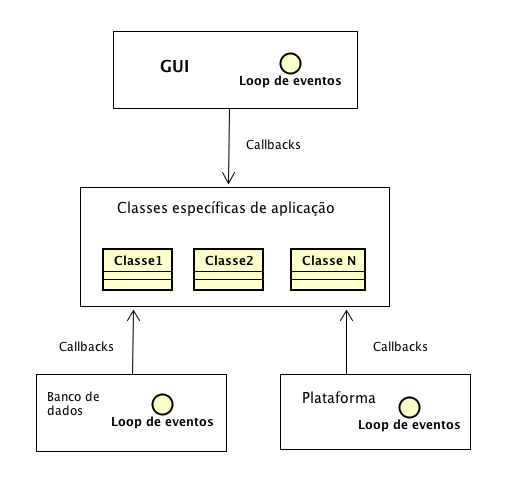
\includegraphics[scale=0.6]{fig/inversaodecontrole.png}
	\caption{Inversão de controle em \textit{framework}. (Adaptado de \cite{sommerville:2013})}
	\label{inversaodecontrole}
\end{figure}

Para especificar o ETL4NoSQL utilizamos a metodologia de desenvolvimento baseada em componentes, pois esta metodologia é fundamentada no reuso e na integração de componentes independentes, cujo encaixa com a necessidade do ETL4NoSQL ser integrado apesar de muitos processos do fluxo de ETL ter funcionalidades independentes. É importante ressaltar também que o desenvolvimento baseado em componentes importa-se com o reuso que é uma característica fundamental para oferecer a flexibilidade necessária ao ETL4NoSQL.

No que diz respeito a \textit{frameworks}, o ETL4NoSQL encaixa-se na categoria de aplicações corporativas, pois serve como base para aplicações de ETL, incorporando conhecimentos sobre a área de domínio para apoiar o desenvolvimento ao usuário final.




\subsection{Estudo Experimental de Software}

Esta dissertação considera a execução do estudo experimental de \textit{software} para caracterizar, avaliar e propor melhorias ao \textit{framework} ETL4NoSQL. O objetivo principal da aplicação do experimento é definir se o \textit{framework} proposto é uma ferramenta adequada para auxiliar no desenvolvimento de processos de ETL em BDs NoSQL. Os participantes escolhidos foram as principais ferramentas de ETL encontradas na literatura. Os questionários utilizados para a coleta de dados são baseadas nos requisitos mínimos considerados pela literatura para ferramentas de ETL.

Segundo \cite{travassos:2002}, a experimentação é o centro do processo científico, por meio dos experimentos que é possível verificar teorias, explorar fatores críticos e formular novas teorias. O autor reforça ainda a necessidade de avaliar novas invenções e sugestões em comparação com as existentes.

Para \cite{wohlin:2000}, existem quatro métodos relevantes para experimentação em Engenharia de \textit{Software}: científico, de engenharia, experimental e analítico. 

O paradigma indutivo, ou método científico, observa o mundo, pode ser utilizado quando se quer entender o processo, produto de \textit{software} e ambiente. Ele mede e analisa, verifica as hipóteses do modelo ou teoria.  Já o método de engenharia observa as soluções existentes, é uma abordagem baseada na melhoria evolutiva, modifica modelos de processos ou produtos de \textit{softwares} existentes com propósito de melhorar os objetos de estudo. O método experimental é uma abordagem baseada na melhoria revolucionária. Ela sugere um modelo, não necessariamente baseado em um existente, aplica o método qualitativo e/ou quantitativo, faz a experimentação, analisa e repete o processo. Por fim, o método analítico sugere uma teoria formal, um método dedutivo que oferece uma base analítica para o desenvolvimento de modelos (\cite{travassos:2002}).

\cite{travassos:2002} sugere que a abordagem mais apropriada para a experimentação na área de Engenharia de \textit{Software} seja o método experimental, pois considera a proposição e avaliação do modelo com os estudos experimentais.

Os principais objetivos relacionados à execução de um estudo experimental de \textit{software} são: caracterização, avaliação, previsão, controle e melhoria a respeito de produtos, processos, recursos, modelos e teorias. Os elementos principais do experimento são: as variáveis, objetos, participantes, o contexto do experimento, hipóteses e o tipo de projeto do experimento.

\section{Trabalhos Correlatos}

\noindent Esta seção apresenta os principais \textit{frameworks} correlatos a este trabalho encontrados na literatura, bem como os descreve demonstrando suas características, seus pontos positivos e negativos.



\subsection{ARKTOS II}

O principal objetivo do ARKTOS II é facilitar a modelagem dos processos de ETL, de forma que o usuário define a fonte dos dados e o destino, os participantes e o fluxo de dados do processo. Como ilustrado na figura \ref{arktosii}, o usuário pode desenhar atributos e parâmetros, conectá-los ao seu esquema de dados, criar relacionamentos e desenhar arestas de um nó para outro de acordo com a arquitetura do grafo (\cite{vassiliadis:2005}).


\begin{figure}[h]
	\centering
	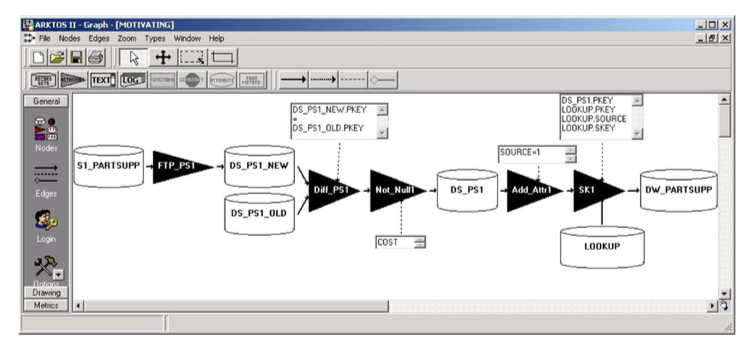
\includegraphics[scale=0.5]{fig/arktosii.png}
	\caption{Exemplo da Ferramenta ARKTOS II em uso (Adaptado de \cite{vassiliadis:2005})}
	\label{arktosii}
\end{figure}

A customização no ARKTOS II é oferecida pela reusabilidade de seus \textit{templates}. Os processos são armazenados em um repositório implementado em um banco de dados relacional. Os autores do ARKTOS II ainda pretendem melhorar a ferramenta permitindo mais formatos de dados como XML.


\subsection{PygramETL}

PygramETL é um \textit{framework} programável para desenvolvedores de ETL. Ele oferece a funcionalidade para desenvolver ETL demonstrando como deve-se iniciar um projeto. O propósito da ferramenta é facilitar a carga dos dados no DW gerenciado por banco de dados relacionais (SGBDs). Focando nos SGBDs relacionais como destino torna o desenvolvimento simples, não considerando outros tipos de estrutura de dados e a integração deles. Dessa forma, o PygramETL oferece suporte apenas para SGBDs relacionais (\cite{thomsen:2009}).

\subsection{ETLMR}

ETLMR é um framework de ETL que utiliza \textit{MapReduce} para atingir escalabilidade. Ele suporta esquemas de DW como o esquema estrela, o \textit{snowflake}, e o \textit{slowly changing dimensions} (\cite{liu:2011}). 

A figura \ref{etlmr} ilustra o fluxo de dados usando o ETLMR e MapReduce. O processamento da dimensão é feito em uma tarefa do MapReduce, e o processamento do fato é feito por outra tarefa MapReduce. A tarefa MapReduce gera um número de tarefas map/reduce paralelas para processar a dimensão ou o fato. Cada tarefa consiste em inúmeros passos, incluindo a leitura dos dados no sistema de arquivos distribuído (DFS - distributed file system), execução da função de mapeamento, particionamento, combinação do mapeamento de saída, execução da função reduce e escrita dos resultados (\cite{liu:2011}).

\begin{figure}
	\centering
	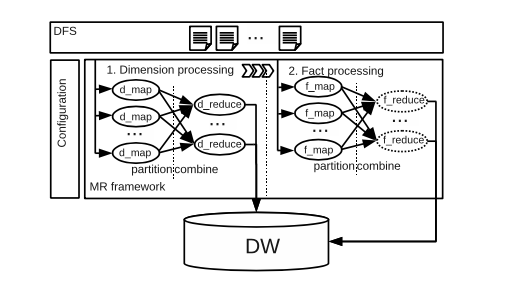
\includegraphics[scale=0.9]{fig/etlmr.png}
	\caption{Fluxo de dados ETL no framework MapReduce (Adaptado de \cite{liu:2011})}
	\label{etlmr}
\end{figure}

O ETLMR possui inúmeras contribuições, ele permite construir dimensões de ETL em alto nível processando os esquemas estrela, snowflake, SCDs e dimensões de dados intensivos. Pelo fato dele utilizar MapReduce, ele pode automaticamente processar mais de um nó enquanto ao mesmo tempo fornece a sincronização dos dados através dos nós. Além da escalabilidade, ele oferece alta tolerância à falhas, possui código aberto e é fácil de usar com um único arquivo de configuração executando todos os parâmetros.

O principal objetivo do ETLMR é otimizar o tempo de processamento dos processos de ETL por meio do \textit{framework} MapReduce. Porém, não há nada a respeito de como auxiliar na modelagem dos processos de ETL.

\subsection{CloudETL}

O \textit{framework} CloudETL é uma solução para processos de ETL que usa \textit{Hadoop} para paralelizar os processos de ETL e \textit{Hive} para processar os dados de forma distribuída. Para o CloudETL o \textit{Hadoop} é a plataforma de execução dos processos de ETL e o \textit{Hive} é o sistema de armazenamento. Conforme a figura \ref{cloudetl}, os componentes do CloudETL são as APIs (Interfaces de Programação de Aplicação), um conjunto de elementos para efetuar as transformações nos dados, identificados como ETL \textit{transformers}, e um gerenciador de tarefas que controla a execução das tarefas submetidas ao \textit{Hadoop}. 

O CloudETL fornece suporte de alto nível em ETL para construção de diferentes esquemas de DW, como esquema estrela, \textit{snowflake} e SCD (\textit{slowly changing dimensions}). Ele facilita a implementação de processos de ETL em paralelo e aumenta a produtividade do programador significativamente. Esta abordagem facilita as atualizações de SCDs em um ambiente distribuído (\cite{liu:2013}).

\begin{figure}[h]
	\centering
	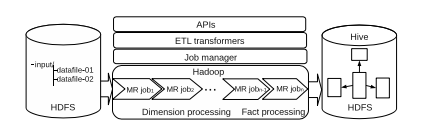
\includegraphics[scale=0.9]{fig/cloudetl.png}
	\caption{Arquitetura do CloudETL (Adaptado de \cite{liu:2013})}
	\label{cloudetl}
\end{figure}

O CloudETL é uma alternativa quando o problema é o processamento de um grande volume de dados por possuir a propriedade de processamento distribuído, porém não oferece nenhum suporte para modelagem de processos de ETL ficando a cargo do programador ou da equipe responsável pelo projeto de DW. 


\subsection{P-ETL}

P-ETL (Parallel - ETL) foi desenvolvido utilizando o \textit{framework} Hadoop com o paradigma MapReduce. Ele oferece duas maneiras de ser configurado: por meio de uma GUI (\textit{Graphical User Interface}) ou um arquivo de configuração XML. A figura \ref{petl} mostra a interface gráfica de configuração do P-ETL, ela é organizada em três abas: \textit{Extract, Transform, Load}; e uma parte para parâmetros avançados. 

O processo de ETL do \textit{framework} inicia-se na aba \textit{Extract}, as configurações fornecidas pelas outras abas dependem desta primeira, principalmente o formato dos dados da fonte de dados e sua estrutura. O primeiro passo da fase de extração é localizar a fonte de dados.  O arquivo base do P-ETL é no formato "csv" (\textit{Comma Separated Values}). Ele converte a fonte para o formato "csv" permitindo a entrada dos dados em vários formatos. Para acelerar a carga dos dados da fonte no HDFS (formato utilizado pelo \textit{Hadoop}), o P-ETL permite o usuário comprimi-los. A respeito da partição, o usuário pode escolher o tipo de partição (\textit{single, Round Robin, Round Robin by block}) e o número de dados por partição, além disso, ele pode configurar a extração pela quantidade de tuplas (por linhas ou blocos). A aba \textit{Transform} permite o usuário escolher um lista de funções para transformação, cada função deve ser especificamente configurada (condições, expressões, entradas, etc.), assim, as funções são executadas na ordem que foram inseridas. E finalmente, a aba \textit{Loading} permite configurar as tarefas de carga e incluir o destino dos dados (\textit{data warehouse, datamart, etc.}), os dados são comprimidos antes de serem carregados no HDFS e o separados no formato "csv" (\cite{bala:2014}).

\begin{figure}[h]
	\centering
	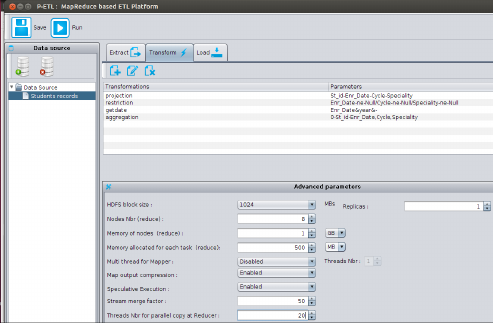
\includegraphics[scale=0.9]{fig/petl.png}
	\caption{Interface de configuração do P-ETL (Adaptado de \cite{bala:2014})}
	\label{petl}
\end{figure}

O P-ETL usa principalmente dois módulos do \textit{framework} Apache Hadoop: (i) HDFS para o armazenamento distribuído e a alta vazão para o acesso aos dados das aplicações, e (ii) MapReduce para processar paralelamente. Futuramente, o P-ETL pretende adicionar outras funções de transformação para realizar processos mais complexos, e oferecer um ambiente na nuvem, mais precisamente, virtualizar e transformá-lo numa arquitetura orientada à serviço (SOA - \textit{Service Oriented Architecture}) (\cite{bala:2014}).


\subsection{Big-ETL}

\cite{bala:2015} propõe em seu trabalho uma abordagem chamada Big-ETL, no qual define que funcionalidades de ETL podem ser executadas em \textit{cluster} utilizando o paradigma MapReduce (MR). O Big-ETL permite paralelizar e distribuir o processo de ETL em dois níveis: o processo de ETL (nível de granularidade maior - todo fluxo de ETL), e a funcionalidade de ETL (nível de granularidade menor - por exemplo, junção de tabelas); dessa forma, melhorando o desempenho. Para testar a abordagem proposta, o autor utilizou o P-ETL com intuito de melhorar a ferramenta definindo o processo de ETL (nível de granularidade maior), e a funcionalidade de ETL (nível de granularidade menor) como níveis para o experimento, demonstrando ser uma boa alternativa para melhorar o desempenho nos processos de ETL.

Futuramente os autores pretendem apresentar um \textit{benchmark} no qual comparará quatro abordagens: processo de ETL centralizado; processo de ETL distribuído, Big-ETL e uma abordagem híbrida.

\subsection{FramETL}

O FramETL é um \textit{framework} para desenvolvimento de aplicações ETL. Ele oferece um ambiente programável e integrado para modelagem e execução de processos de ETL utilizando uma linguagem de programação. O autor utilizou conceitos de \textit{frameworks} como flexibilidade, extensibilidade, reuso e inversão de controle para o desenvolvimento do FramETL. Por meio desses conceitos, utilizando o \textit{framework}, o autor aplicou sua solução para construções de duas aplicações de ETL. Porém, \cite{silva:2012} não fez uso de SGBDs NoSQL, pois o foco de sua ferramenta não era lidar com esses tipos de SGBDs.

\subsection{Outras Ferramentas}

Esta subseção apresenta outras ferramentas de ETL presentes no mercado e na literatura, mas que não possuem foco em SGBDs NoSQL apesar de darem algum tipo de suporte à eles.

\subsubsection{Pentaho}

Pentaho Data Integration (conhecido também por \textit{\textbf{Kettle}}) é uma ferramenta \textit{open source} para aplicações de ETL. Ela é composta basicamente por quatro elementos: extração de diferentes fontes de dados, transporte de dados, transformação dos dados e carga em \textit{data warehouse}. O \textit{Kettle} pode ser implementado em um único nó, bem como na nuvem, ou em \textit{cluster}. Ele pode carregar e processar \textit{big data} de várias formas oferecendo flexibilidade e segurança (\cite{mali:2015}, \cite{ETLtools}, \cite{pentaho}). Porém, por ser uma ferramenta genérica ela é de difícil customização, e muitas vezes é considerada de difícil utilização por seus usuários, além de ter partes de suas funcionalidades disponíveis apenas em edições comerciais.

\subsubsection{Talend Studio}

\textit{Talend Open Studio} é uma plataforma de integração de dados que possibilita processos de integração, seu monitoramento opera como um gerador de código, produzindo \textit{scripts} de transformação. Ele possui um repositório de metadados no qual fornece os dados (definições e configurações relacionados a cada tarefa) para todos os seus componentes. O Talend Studio é comumente utilizado para migração de dados, sincronização ou replicação das bases de dados  (\cite{mali:2015}, \cite{ETLtools}). 

\subsubsection{CloverETL}

\textit{Clover} é uma ferramenta ETL de código aberto considerada para transformação e integração, limpeza e distribuição de dados em aplicações, banco de dados e \textit{data warehouses}. Ela é baseada em Java e pode ser utilizada em linha de comando e é independente de plataforma (\cite{mali:2015}). Porém, por ter vários recursos sua curva de aprendizagem é alta e muitos desses recursos valiosos estão disponíveis apenas em sua edição comercial.

\subsubsection{Oracle Data Integrator (ODI)}

\textit{Oracle Data Integrator} é uma plataforma de integração de dados que atende diversos requisitos de integração, desde grandes volumes de dados até o carregamento em \textit{batch}. As bases de dados de origem e destino podem incluir base de dados relacionais, arquivos XML, tabelas \textit{Hive, Hbase}, arquivos \textit{HDFS}, entre outros. Os usuários podem inserir filtros, junções, agregações, e outros componentes de transformação (\cite{silva:2016}). Porém, o ODI é uma ferramenta comercial e não permite a customização de suas aplicações.

\section{Considerações Finais}

Este capítulo discorreu a respeito dos principais assuntos abordados nesta dissertação, bem como as ferramentas de ETL encontradas na literatura. A maioria delas foca no desempenho ao lidar com grandes volumes de dados e BDs NoSQL. A ferramenta P-ETL (\cite{bala:2014}) apresentou um arquivo "csv" como alternativa para exportar diversos tipos de dados, porém não há um enfoque em BDs NoSQL. A abordagem PygramETL (\cite{thomsen:2009}) facilita a carga de dados, mas lida apenas com SGBDs relacionais. Outras ferramentas como o ETLMR, CloudETL, BigETL utilizam processamento paralelo e distribuído para facilitar a execução dos processos de ETL apenas, deixando a cargo do projetista de ETL a modelagem dos processos.

O capítulo seguinte irá apresentar os componentes de ETL4NoSQL, o \textit{framework} programável, flexível e integrado proposto por esta dissertação como uma alternativa para sanar a dificuldade de modelar, executar e reutilizar processos de ETL em BDs NoSQL.

%Para suportar processos de ETL em BDsNoSQL, propomos um \textit{framework} integrado, flexível e programável de ETL para BDs NoSQL que permite o uso do processamento distribuído/paralelo e a integração das diversas bases de dados existentes por se tratar de um \textit{framework} baseado em componentes.  
%\chapter{Trabalhos Correlatos}

\noindent Este capítulo aborda os trabalhos que são correlatos a esta pesquisa, bem como descreve como estes trabalhos diferem do realizado
por esta pesquisa.
\clearpage

\section{Ferramentas de ETL}



\subsection{ARKTOS II}
ARKTOS II: modela os processos de ETL

\subsection{PygramETL}
PygramETL: 

\subsection{ETLMR}
ETLMR é um framework de ETL que utiliza \textit{MapReduce} para atingir escalabilidade. Ele suporta esquemas de DW como o esquema estrela, o \textit{snowflake}, e o \textit{slowly changing dimensions} \cite{liu:2011}. 

A figura \ref{etlmr} 

\begin{figure}[h]
	\centering
	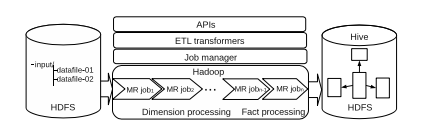
\includegraphics[scale=0.7]{fig/cloudetl.png}
	\caption{Fluxo de dados ETL no framework MapReduce (Adaptado de \cite{liu:2011})}
	\label{etlmr}
\end{figure}


\subsection{CloudETL}

O framework CloudETL é uma solução para processos de ETL que usa \textit{Hadoop} para paralelizar fluxos de ETL e \textit{Hive} para processar os dados de forma distribuída. Para o CloudETL o \textit{Hadoop} é a plataforma de execução dos processos de ETL e o \textit{Hive} é o sistema de armazenamento. Conforme a figura \ref{cloudetl}, os componentes do CloudETL são as APIs (interfaces de programação de aplicação), um conjunto de elementos para efetuar as transformações nos dados identificados como ETL \textit{transformers}, e um gerenciador de tarefas que controla a execução das tarefas submetidas ao \textit{Hadoop}. 

CloudETL fornece suporte de alto nível em ETL para construção de diferentes esquemas de DW, como esquema estrela, \textit{snowflake} e SCD (\textit{slowly changing dimensions}). Ele facilita a implementação de processos de ETL em paralelo e aumenta a produtividade do programador significativamente. Esta abordagem facilita as atualizações de SCDs em um ambiente distribuído \cite{liu:2013}.

\begin{figure}[h]
	\centering
	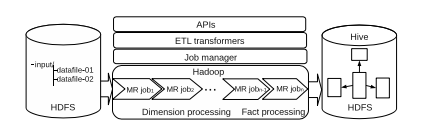
\includegraphics[scale=0.7]{fig/cloudetl.png}
	\caption{Arquitetura do CloudETL (Adaptado de \cite{liu:2013})}
	\label{cloudetl}
\end{figure}

O CloudETL é uma alternativa quando o problema é o processamento de um grande volume de dados por possuir a propriedade de processamento distribuído, porém não oferece nenhum suporte para modelagem de processos de ETL ficando a cargo do programador ou da equipe responsável pelo projeto de DW. 


\subsection{P-ETL}
P-ETL:

\subsection{Big-ETL}
Big-ETL: Foca na paralelização e distribuição.

\subsection{FramETL}
FramETL

\subsection{Pentaho}
Pentaho

\subsection{Talend Studio}
Talend Studio for Data Integration

\subsection{CloverETL}
CloverETL

\subsection{Oracle Data Integrator (ODI)}
Oracle Data Integrator (ODI)
\chapter{O Framework ETL4NoSQL}
% ---
Neste capítulo são apresentados os conceitos do \textit{framework} ETL4NoSQL, que consiste numa plataforma de \textit{software} para desenvolvimento de sistemas de ETL, mais especificamente uma ferramenta que auxilia a construção de processos de ETL buscando apoiar a modelagem e o desempenho dos processos. 

O ETL4NoSQL oferece um ambiente com componentes integrados para modelar processos de ETL e implementar funcionalidades utilizando uma linguagem de programação independente de uma GUI (\emph{Graphical User Interface} - Interface Gráfica do Usuário).


Para a especificação do \textit{framework} proposto neste trabalho, foram elencados os requisitos de \textit{software} utilizando a abordagem de desenvolvimento baseado em componentes, fundamentada no estudo de \cite{cheesman:2001}. Neste estudo, temos a separação entre a modelagem do domínio e da especificação. A modelagem de domínio consiste na definição dos casos de uso, do modelo conceitual e do modelo comportamental. Já a modelagem de especificação é segmentada em três partes, a parte de identificação de componentes, de interação entre os componentes e a especificação de componentes.  

%definidas as estruturas de dados dos ambientes de origem, destino e da área de processamento de dados e suas respectivas linguagens de manipulação de dados, e também, as principais funcionalidades dos sistemas de ETL, chamados mecanismos de ETL. Para realizar os processos de ETL, por meio de seus mecanismos, foi definido um controlador de operações que é capaz de se comunicar com os ambientes e os mecanismos de ETL. 

A seguir, são detalhados os requisitos de \textit{software}, os modelo de domínio, os modelos de especificação, as especificações dos componentes, o ambiente de implementação e as interfaces de programação do ETL4NoSQL.

% a arquitetura do sistema e a estrutura dos componentes utilizados no desenvolvimento do framework.

\clearpage
% ---
\section{Requisitos de software do ETL4NoSQL}


Requisitos de \textit{software} são descrições de como o sistema deve se comportar, definidos durante as fases iniciais do desenvolvimento do sistema como uma especificação do que deveria ser implementado (\cite{sommerville:2013}). Os requisitos podem ser divididos em funcionais e não funcionais, onde o primeiro descreve o que o sistema deve fazer, ou seja, as transformações a serem realizadas nas entradas de um sistema, a fim de que se produzam saídas, já o outro expressa as características que este \textit{software} vai apresentar (\cite{sommerville:2013}). 

O ETL4NoSQL é um \textit{framework} que tem como principal objetivo auxiliar na criação de processos de ETL ao se utilizar principalmente BDs NoSQL. Um sistema de \textit{software} pode ter seus dados armazenados em BDs relacionais, que seguem o modelo entidade e relacionamento, ou não relacionais, no qual possui pouca definição de esquema, não seguem um modelo específico e são regularmente chamados de BDs NoSQL (\cite{fowler:2013}). Os BDs NoSQL possuem quatro paradigmas frequentemente utilizados: Chave-Valor, Família de Colunas, Documentos e Grafo (\cite{fowler:2013}).

Os BDs relacionais utilizam uma linguagem de gerenciamento de dados padrão conhecida por SQL (Structure Query Language) (\cite{fowler:2013}), porém os BDs NoSQL não possuem uma linguagem em comum, como os BDs relacionais, cada estrutura de armazenamento possui sua própria linguagem de gerenciamento de dados (\cite{fowler:2013}). Por isso, é essencial que haja um componente que seja capaz de fazer a leitura diretamente da fonte de dados e um componente que também possa carregar esses dados diretamente no seu destino, independente do seu tipo, saber se é um arquivo texto, um arquivo XML, SGBD relacional, SGBD NoSQL, entre outros. Um componente tem como uma de suas definições ser uma unidade de \textit{software} independente, que encapsula a sua implementação, e oferece serviços por meio de suas interfaces (\cite{itana:2005}).

Outra importante características ao especificar o uso do ETL4NoSQL são os processos de ETL, que possuem quatro etapas básicas: extração, limpeza/transformação e carga (\cite{kimball:2004}). O fluxo do processo de ETL inicia-se com a extração dos dados a partir de uma fonte de dados. A começar da extração, é possível que um componente passe os dados para uma \acp{apd}, onde é permitido modelar os dados executando processos de limpeza e transformação por meio de mecanismos como de junção, filtro, união, agregação e outros. E finalmente, os dados são carregados em uma estrutura de dados destino.

Dessa forma, o ETL4NoSQL possui um componente que permite a leitura dos dados de diversos SGBDs NoSQL, de arquivos textuais, além dos SGBDs relacionais. Outro componente que permite a execução dos mecanismos de ETL, este componente também faz uso de componentes para o gerenciamento da execução dos processos, bem como a construção da sequência dos processos de ETL e a escolha do tipo de processamento. O ETL4NoSQL é composto também de um componente que permite carregar diretamente os dados no destino independente do seu tipo. No quadro \ref{requisitos} é apresentado os principais requisitos elencados do ETL4NoSQL. Foi definido como importante as prioridades que são imprescindíveis para o desenvolvimento e funcionamento do \textit{framework}, e desejável as funcionalidades que aprimoram o uso do \textit{framework}, porém não interferem no seu principal objetivo.

\begin{table}[h]
	\centering
	\caption{Requisitos do ETL4NoSQL}
	\label{requisitos}
	\begin{tabular}{|p{3cm}| p{10cm}| p{2cm} |}
		\hline
		Funcionalidade & Requisito & Prioridade\\
		\hline
		Suporte à plataforma &  Ser independente de plataforma & Importante\\
		\hline
		Suporte à fonte &  Ser capaz de ler diretamente da fonte de dados, independente do seu tipo, saber se é uma fonte RDBMS, arquivo de texto, XML ou NoSQL. & Importante\\
		\hline
		Suporte ao destino & Ser capaz de carregar diretamente os dado no destino, independente do  seu tipo, saber se o destino é RDBMS, arquivo de texto, XML ou NoSQL. & Importante\\
		\hline
		Suporte à modelagem & Apoiar na extração de dados de múltiplas fontes, na limpeza dos dados, na transformação, agregação, reorganização e operações de carga. & Importante\\
		\hline
		Paralelismo &Apoiar as operações de vários segmentos e execução em paralelo, internamente. A ferramenta deve ser capaz de distribuir tarefas entre múltiplos servidores. & Importante\\
		\hline
		Programável &Apoiar o agendamento de tarefas de ETL e ter suporte para programação em linha de comandos usando programação externa. & Importante\\
		\hline
		Reutilização & Apoiar a reutilização dos componentes do framework e da lógica das transformações para evitar a reescrita. & Importante\\
		\hline
		Apoio ao nível de debugging & Apoiar o tempo de execução e a limpeza da lógica de transformação. O usuário deve ser capaz de ver os dados antes e depois da transformação. & Desejável\\
		\hline
		Implementação & Suportar a capacidade de agrupar os objetos ETL e implementá-los em ambiente de teste ou de produção, sem a intervenção de um administrador de ETL. & Desejável\\
		\hline
		Garantia de Qualidade & Ser capaz de estabelecer processos, métricas e avaliações que possibilitem e garantam a qualidade de software. & Desejável\\
		\hline
		
		
	\end{tabular}
\end{table}


\section{Modelagem do Domínio de ETL4NoSQL}

A modelagem do domínio de ETL4NoSQL é apresentada a seguir por meio de seus três modelos: modelo conceitual, modelo de casos de uso e modelo de comportamento.

\subsection{Modelo Conceitual}

Os conceitos de aplicações ETL, identificados para o ETL4NoSQL, são: Fonte, Destino, Modelagem, Processamento, Operações, ProcessamentoDistribuído e ProcessamentoCentralizado. O modelo conceitual pode ser visualizado na figura \ref{modeloconceitual}.

\begin{figure}[h]
	\centering
	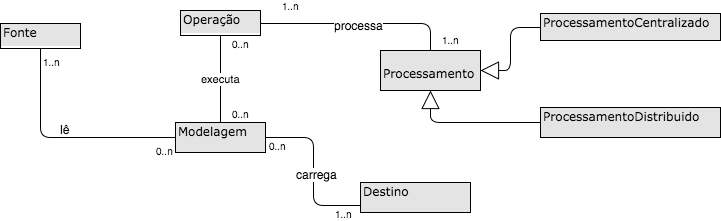
\includegraphics[scale=0.6]{fig/modeloconceitual.png}
	\caption{Modelo conceitual do ETL4NoSQL}
	\label{modeloconceitual}
\end{figure}

A entidade Modelagem faz a leitura de uma ou mais Fontes de dados, executa nenhuma ou muitas Operações. As Operações por sua vez são processadas por um ou mais Processamentos de forma a serem Processamentos Centralizados ou Processamentos Distribuídos. E por fim, a Modelagem carrega o resultado das Operações processadas à um ou mais Destinos.

A seguir é apresentado o modelo de casos de uso do ETL4NoSQL.

\subsection{Modelo de Casos de Uso}

Um conjunto de casos de uso foram identificados tais como: Ler fonte de dados, Escrever no destino, Modelar dados, Executar operação e Processar operações. O quadro \ref{casosdeuso} mostra a descrição sucinta de cada caso de uso. Os casos de uso expressam as funcionalidades fundamentais ao desenvolvimento e uso do ETL4NoSQL. Eles permitem ao programador a visão do que é imprescindível ao implementar e determinar as interfaces de sistema e operações do \textit{framework}. 

Para finalizar a modelagem do domínio de ETL4NoSQL, na subseção seguinte é apresentado o modelo comportamental do \textit{framework} proposto neste trabalho.



\begin{table}[h!]
	\centering
	\caption{Modelo de Casos de Uso do ETL4NoSQL}
	\label{casosdeuso}
	\begin{tabular}{|p{14cm}|}
		\hline
			\textbf{Nome:} Ler fonte de dados\\ 
			\textbf{Objetivo:} Fazer a leitura de qualquer tipo de dados a partir de uma fonte de dados.\\ 
			\textbf{Pré-condição:} os parâmetros para permissão de conexão com a fonte de dados devem estar disponíveis.\\ 
			\textbf{Ação:} ler (Fonte)\\ 
		\hline
			\textbf{Nome:} Escrever no destino\\ 
			\textbf{Objetivo:} Fazer a escrita de qualquer tipo de dado a partir do modelo processado pelo ETL4NoSQL em uma base de destino.\\ 
			\textbf{Pré-condição:} os parâmetros para permissão de conexão e escrita com o destino devem estar disponíveis.\\ 
			\textbf{Ação:} escrever (Destino)  \\ 
	\hline
			\textbf{Nome:} Modelar dados\\ 
			\textbf{Objetivo:} Permitir a modelagem dos dados por meio de mecanismos de junção, filtro, união, agregação e outros. \\
			 \textbf{Pré-condição:} os mecanismos de transformação e limpeza devem estar disponíveis para executar a modelagem.\\ 
			 \textbf{Ação:} modelar (Modelagem, Operação)\\ 
	 \hline
	 		\textbf{Nome:} Executar operação\\ 
	 		\textbf{Objetivo:} Armazenar, gerenciar e executar as operações criadas pela ação de modelar.\\
	 		\textbf{Pré-condição:} as operações devem ser criadas previamente pela ação de modelar.\\ 
	 		\textbf{Ação:} executar (Operação, Processamento)\\ 
	 \hline
	 	\textbf{Nome:} Processar operações\\ 
	 	\textbf{Objetivo:} Processar as operações armazenadas de forma centralizada ou distribuída.\\
	 	\textbf{Pré-condição:} as operações precisam estar disponíveis para o processamento.\\ 
	 	\textbf{Ação:} processar (Processamento, Operação)\\ 
	 \hline
	 
	\end{tabular}
\end{table}

\subsection{Modelo Comportamental}

Ao construir o modelo comportamental é possível identificar os conceitos com comportamentos mais relevantes para o negócio, bem como os estados e eventos que disparam as transições entre os estados (\cite{itana:2005}). Dessa forma, o diagrama de estados do ETL4NoSQL é apresentado na figura \ref{diagrama_estado}, nele podemos ver as transições de leitura da fonte de dados, validação e identificação dos dados, assim como o tratamento caso os dados não possam ser identificados. Subsequente a isso, o armazenamento dos dados para o processamento, a criação dos processos de ETL, a escolha da forma de processamento, execução das operações, e também o tratamento para as operações que não puderem ser executadas. Finalmente, pode ser feita a carga dos dados na base de destino seguido da mensagem de tratamento, caso haja sucesso ou não na execução.

\begin{figure}[h!]
	\centering
	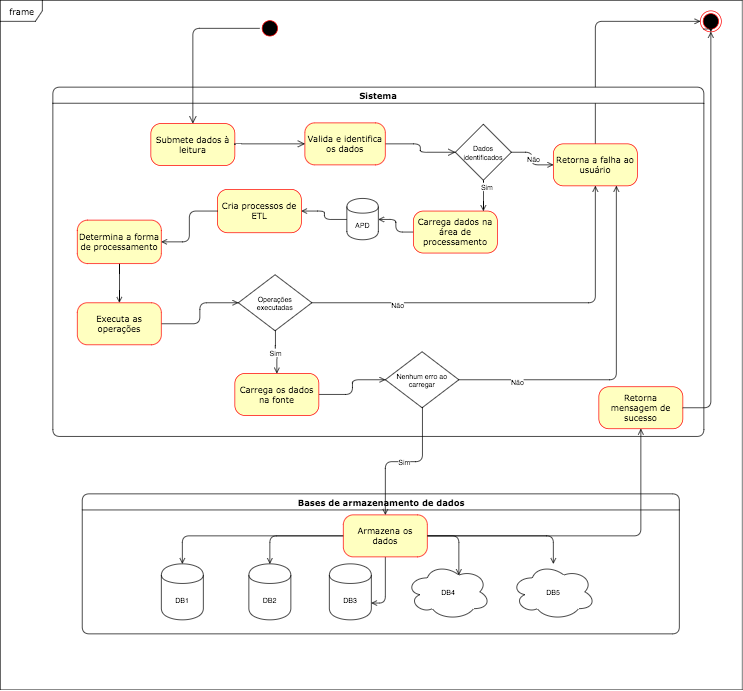
\includegraphics[scale=0.6]{fig/diagrama_estado.png}
	\caption{Diagrama de Estado do ETL4NoSQL}
	\label{diagrama_estado}
\end{figure}

\section{Modelagem da Especificação do ETL4NoSQL}

A modelagem de especificação visa definir, em um nível alto de abstração, os serviços oferecidos pelos componentes (\cite{itana:2005}). Dessa forma, é possível determinar a arquitetura e especificar os componentes. É importante dar ênfase a especificação das interfaces, pois isso contribui para uma clara separação entre os componentes, e também, para assegurar o princípio de encapsulamento de dados e comportamento (\cite{itana:2005}). \cite{cheesman:2001} divide a modelagem da especificação em três estágio, sendo assim, os estágios da modelagem de especificação do ETL4NoSQL são apresentados a seguir.


\subsection{Identificação de Componentes}
Seguindo o modelo de conceitos do negócio e do modelo de casos de uso foi possível identificar as interfaces para os componentes de negócio, as interfaces de sistema para os componentes de sistema e gerar a arquitetura de componentes inicial. As interfaces de negócio são reconhecidas por meio do modelo conceitual,  as interfaces de sistema e operações a partir dos casos de uso.

\subsection{Interfaces de Sistemas}

As interfaces de sistemas do ETL4NoSQL identificadas, por meio do modelo de casos de uso apresentado no quadro \ref{casosdeuso}, foram: IReadData, IWriteData, IModelData, IExeOp e IProcOp. Para especificar as interfaces foi utilizado \acp{OCL} (\cite{warmer:1998}).
\\
\lstset{emph={%  
		context, pre, post%
	},emphstyle={\color{black}\bfseries\underbar}%
}%
\begin{lstlisting}[frame=single, language=Oberon-2]
	context System :: IReadData (source : Fonte)	
	pre:	
	
	Fonte.allInstances@includes(Fonte) 
	Fonte.connection = estabelecido
		
	Fonte.allInstances@includes(Fonte) 
	Fonte.connection = retorna mensagem de erro
	
	Fonte.allInstances@includes(Fonte) 
	Fonte.structureType =  reconhecido	

	Fonte.allInstances@includes(Fonte)
	Fonte.structureType = retorna mensagem de erro	
	
	post:
	
	Fonte. allInstances@includes 
	(f: Fonte | not Fonte.allInstances@pre@includes (f) and	
	Os atributos do objeto f foram inicializados)	
\end{lstlisting}

A partir da especificação foram identificadas as operações: Interface IReadData (Connection(connect), structureType()).

\begin{lstlisting}[frame=single, language=Oberon-2]
context System :: IWriteData (load : Destino)

pre:

Destino.allInstances@includes(Destino) 
Destino.connection = estabelecido

Destino.allInstances@includes(Destino) 
Destino.connection = retorna  erro

Destino.allInstances@includes(Destino)
Destino.structureType = reconhecido

Destino.allInstances@includes(Destino)
Destino.structureType = retorna  erro

Destino.allInstances@includes(Destino) 
Destino.structureType = permissao de escrita

Destino.allInstances@includes(Destino)
Destino.structureType = retorna  erro

post:

Fonte. allInstances@includes (d: Destino | not 
Destino.allInstances@pre@includes (d) and
Os atributos do objeto d foram inicializados)
\end{lstlisting}

As operações identificadas foram: Interface IWriteData (connection(connect), structureType(), allowWrite()).

\begin{lstlisting}[frame=single, language=Oberon-2]
	context System :: IModelData (model : Modelagem; 
	source: Fonte; operation: Operacao)
	
	pre:
	Fonte.allInstances@includes(Fonte) 
	Fonte.connection = estabelecido and  
	Fonte.structureType = reconhecido
	
	Fonte.allInstances@includes(Destino) 
	Fonte.connection = retorna  erro
	
	Operacao.allInstances@includes(Operacao) 
	Operacao.mecanismo = existe
	
	Operacao.allInstances@includes(Operacao) 
	Operacao.mecanismo = retorna erro
	
	Modelagem.allInstances@includes(Modelagem) 
	Modelagem.operacao(dados)
	
	post:
	
	Modelagem. allInstances@includes (m: Modelagem | not 
	Destino.allInstances@pre@includes (m) and
	Os atributos do objeto m foram inicializados
	m foi ligado ao objeto f
	f.Fonte = Fonte
	m foi ligado ao objeto o
	o.Operacao = Operacao
	Todas as operacoes de modelagem foram criadas e 
	armazenadas em um APD)
\end{lstlisting}

As operações identificadas foram: Interface IModelData (readData(CodFonte), createOp(CodOperação, data)).

\begin{lstlisting}[frame=single, language=Oberon-2]
	context System :: IExeOp (model : Modelagem; operation: 
	Operacao, processing: Processamento)
	
	pre:
	Modelagem.allInstances@includes(Modelagem) 
	Modelagem.operacoes = existem 
	
	Operaaoo.allInstances@includes(Operacao) 
	Operacao.executa = retorna  erro
	
	Operacao.allInstances@includes(Operacao) 
	Operacao.manage(operacoes)
	
	post:
	Operacao. allInstances@includes (o: Operacao | not 
	Operacao.allInstances@pre@includes (o) and
	
	Os atributos do objeto o foram inicializados
	o foi ligado ao objeto m
	m.Modelagem = Modelagem
	o foi ligado ao objeto p
	p.Processamento = Processamento
	Todas as operacoes escalonadas e estao pronta para 
	o processamento)

\end{lstlisting}

As operações identificadas foram: Interface IExeOp (modelOperation(CodModelagem), operationManagement())

\begin{lstlisting}[frame=single, language=Oberon-2]
	context System :: IProcOp (operation: Operacao, 
	processing: Processamento)
	
	pre:
	Operacao.allInstances@includes(Operacao) 
	Operacao.toExec = pronto
	
	Processamento.allInstances@includes(Processamento) 
	Processamento.typeProc(tipoProcessamento)
	
	post:
		
	Processamento. allInstances@includes (m: Processamento 
	| not Destino.allInstances@pre@includes (p) and
	
	Os atributos do objeto p foram inicializados
	p foi ligado ao objeto o
	o.Operacao = Operacao
	- Foi gerado o processamento das operacoes de acordo 
	com o tipo escolhido)

\end{lstlisting}

As operações identificadas foram: Interface IProcOp (process(CodOperação), typeProc(tipoProcessamento))

\subsection{Interfaces de Negócio}

Para definir as dependências no modelo \cite{cheesman:2001}, identificam o conceito de tipos principais, sendo estes tipos que possuem existência independente.
No ETL4NoSQL foi possível identificar quatro tipos principais: Fonte, Modelagem, Operação e Processamento. Para cada tipo principal foi possível definir uma interface de negócio, como é apresentado na figura \ref{modelo_negocio}.

\begin{figure}[h]
	\centering
	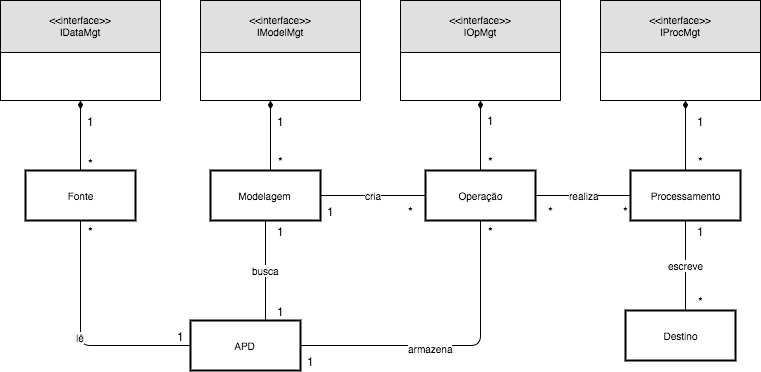
\includegraphics[scale=0.58]{fig/modelo_negocio.png}
	\caption{Definição de interfaces do modelo de negócio do ETL4NoSQL}
	\label{modelo_negocio}
\end{figure}

\subsection{Especificação da Arquitetura do Componente}

\cite{sommerville:2013}, define o projeto de arquitetura como um processo criativo em que se tenta organizar o sistema de acordo com os requisitos funcionais e não funcionais. Um estilo de arquitetura é um padrão de organização de sistema (\cite{shaw:1996}, \cite{sommerville:2013}), como uma organização cliente-servidor ou uma arquitetura em camadas. Porém, a arquitetura não necessariamente utilizará apenas um estilo, a maioria dos sistemas de médio e grande porte utilizam vários estilos. Para \cite{shaw:1996}, há três questões a serem definidas na escolha do projeto de arquitetura, a primeira é a escolha da estrutura, cliente-servidor ou em camadas, que permita atender melhor aos requisitos. A segunda questão é a respeito da decomposição dos subsistemas em módulos ou em componentes. E por fim, deve-se tomar a decisão de sobre como a execução dos subsistemas é controlada. A descrição da arquitetura pode ser representada graficamente utilizando modelos informais e notações como a UML (\cite{clements:2002}, \cite{sommerville:2013}). Para o ETL4NoSQL, cada componente foi associado à sua interface de negócio identificada e uma interface de gerenciamento foi separada das outras interfaces de negócio, como pode ser visto na figura \ref{arquitetura}.

\begin{figure}[h]
	\centering
	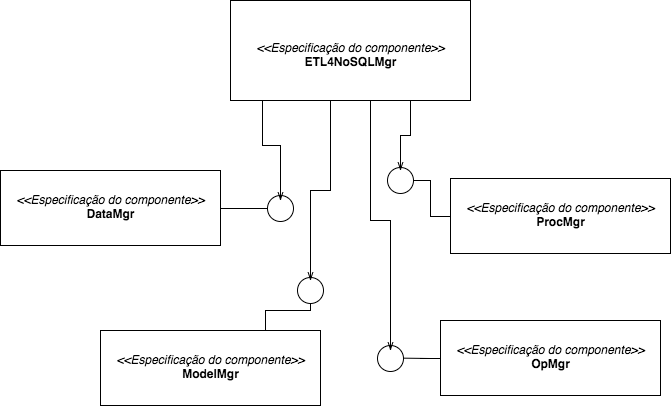
\includegraphics[scale=0.5]{fig/arquitetura_comp.png}
	\caption{Especificação da arquitetura do componente de ETL4NoSQL}
	\label{arquitetura}
\end{figure}

\section{Interação entre Componentes}

Esta etapa é detalhada, em termos de interações, utilizando diagramas de colaboração. Dessa forma, apresentamos os diagramas de colaboração para as interações do ETL4NoSQL na seção a seguir.

\subsection{Operações da interface de negócio}

As operações de negócio são identificadas quando as interações forem analisadas para cada interface do sistema. Analisando as pré e pós-condições das operações de interface do sistema identificadas anteriormente foi possível detalhar usando diagramas de colaboração as interações necessárias para efetuar as operações do ETL4NoSQL. Os diagramas de cada operação podem ser visto nas figuras \ref{colaboracao1}, \ref{colaboracao2}, \ref{colaboracao3}, \ref{readData}, \ref{createOp}, \ref{createOp}, \ref{modelOperation}, \ref{operationManagement} e \ref{process}.

A conexão com a fonte de dados é estabelecida (figura \ref{colaboracao1}).

\begin{figure}[h!]
	\centering
	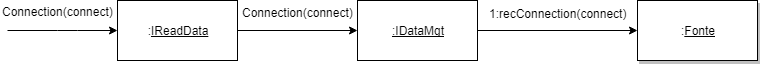
\includegraphics[scale=0.5]{fig/colaboracao1.png}
	\caption{Diagrama de colaboração para conectar à base de fonte de dados}
	\label{colaboracao1}
\end{figure}

A estrutura de dados da fonte é reconhecida (figura \ref{colaboracao2}).

\begin{figure}[h!]
	\centering
	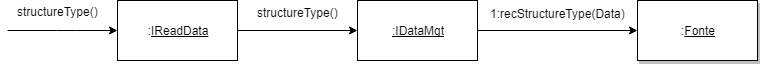
\includegraphics[scale=0.5]{fig/colaboracao2.png}
	\caption{Diagrama de colaboração para verificar a estrutura de dados}
	\label{colaboracao2}
\end{figure}

A escrita na base de dados destino é permitida (figura \ref{colaboracao3}).

\begin{figure}[h!]
	\centering
	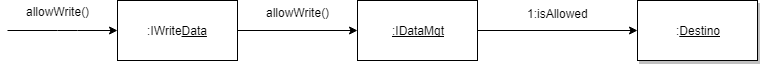
\includegraphics[scale=0.5]{fig/colaboracao3.png}
	\caption{Diagrama de colaboração para verificar se existe permissão de escrita na base de dados destino}
	\label{colaboracao3}
\end{figure}

A leitura dos dados da fonte é feita e armazenada na área de processamento de dados figura (\ref{readData}).

\begin{figure}[h!]
	\centering
	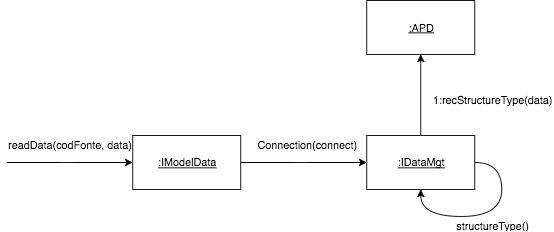
\includegraphics[scale=0.5]{fig/readData.png}
	\caption{Diagrama de colaboração para leitura dos dados da fonte}
	\label{readData}
\end{figure}

Após a leitura dos dados da fonte é possível a criação das operações por meio dos mecanismos existentes (figura \ref{createOp}).

\begin{figure}[h!]
	\centering
	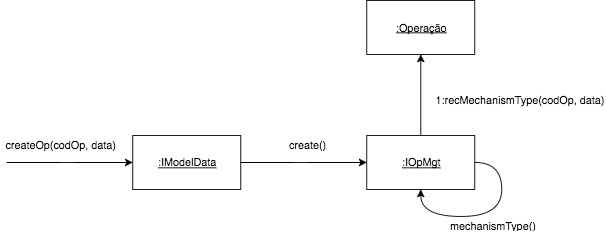
\includegraphics[scale=0.5]{fig/createOp.png}
	\caption{Diagrama de colaboração criação das operações de ETL}
	\label{createOp}
\end{figure}

Com as operações criadas, deve-se colocá-las em ordem de execução (figura \ref{modelOperation}).

\begin{figure}[h!]
	\centering
	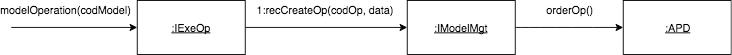
\includegraphics[scale=0.5]{fig/modelOperation.png}
	\caption{Diagrama de colaboração modelar as operações criadas}
	\label{modelOperation}
\end{figure}

É possível também que as operações sejam apagadas e alteradas (figura \ref{operationManagement}).

\begin{figure}[h!]
	\centering
	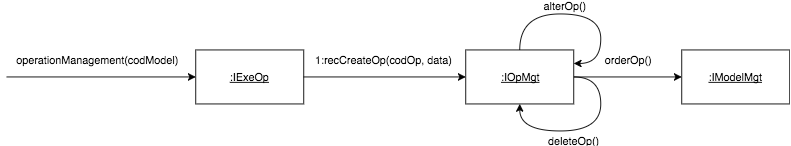
\includegraphics[scale=0.5]{fig/operationManagement.png}
	\caption{Diagrama de colaboração para gerenciar as operações}
	\label{operationManagement}
\end{figure}

Com as operações criadas é possível processá-las de forma a escolher o tipo de processamento (centralizado ou distribuído) (figura \ref{process}).

\begin{figure}[h!]
	\centering
	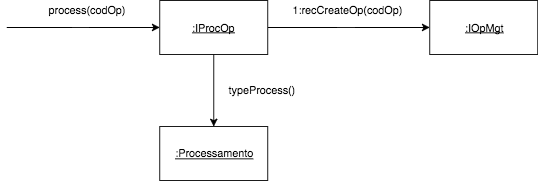
\includegraphics[scale=0.5]{fig/process.png}
	\caption{Diagrama de colaboração para processar as operações}
	\label{process}
\end{figure}

\section{Especificação de Componentes}

Posteriormente à definição das interfaces de negócio, é possível detalhá-las. Para cada interface, as operações são especificadas com suas assinaturas, pré e pós-condições.

\begin{alltt}
	
	\textbf{context} IDataMgt :: connection(connect):Fonte
		\textbf{pré:}
		- Existe um parâmetro de conexão "connect"
		- Existe uma fonte para ser conectada
		\textbf{pós:}
		- A conexão com a fonte é estabelecida ou não
		- Recebe uma mensagem de conexão bem sucedida ou erro

	\textbf{context} IDataMgt :: strutuctureType():Fonte
		\textbf{pré:}
		- A conexão com a fonte foi bem sucedida
		\textbf{pós:}
		- A estrutura de dados é reconhecida ou não
		- Retorna mensagem de sucesso ou erro
		
	\textbf{context} IDataMgt :: allowWrite():Destino
		\textbf{pré:}
		- A conexão com o destino foi bem sucedida
		\textbf{pós:}
		- A base de dados destino permite escrita ou não
		- Retorna mensagem de sucesso ou erro
	
	\textbf{context} IModelMgt :: readData(codFonte, data):APD
		\textbf{pré:}
		- A conexão com a fonte foi bem sucedida
		- A estrutura de dados é reconhecida
		- Existe um parâmetro de busca "data" válido para 
		estrutura de dados reconhecida
		\textbf{pós:}
		- A leitura dos dados é realizada ou não
		- Retorna os dados em uma APD ou uma mensagem de erro
		
	\textbf{context} IModelMgt :: createOp(codOp, data):Operação
		\textbf{pré:}
		- Existe o mecanismo desejado para a criação da operação
		- Existe um parâmetro "data" com os dados a serem 
		usados na operação
		\textbf{pós:}
		- A operação é criada ou não
		- Retorna o codOp ou uma mensagem de erro
		
	\textbf{context} IOpMgt :: modelOperation(codModel)
		\textbf{pré:}
		- Existem operações criadas na APD (codModel)
		\textbf{pós:}
		- As operações são ordenadas para execução
		
	\textbf{context} IOpMgt :: operationManagement(codModel)
		\textbf{pré:}
		- Existem operações criadas na APD (codModel)
		\textbf{pós:}
		- As operações foram alteradas, apagadas ou não
		- Retorna mensagem de sucesso ou erro
	
	\textbf{context} IProcMgt :: process(codOp)
		\textbf{pré:}
		- Existe a operação (codOp)
		- Foi escolhido o tipo de processamento (centralizado ou distribuído)
		\textbf{pós:}
		- A operação foi processada ou não
		- Retorna mensagem de sucesso ou erro
		
			
\end{alltt}

Depois das operações terem sido especificadas, o diagrama de especificação das interfaces foi criado e está representado na figura \ref{interfaces}. Essas especificações referem-se ao uso dos componentes. Elas representam o que o usuário precisa saber sobre os componentes.

\begin{figure}[h!]
	\centering
	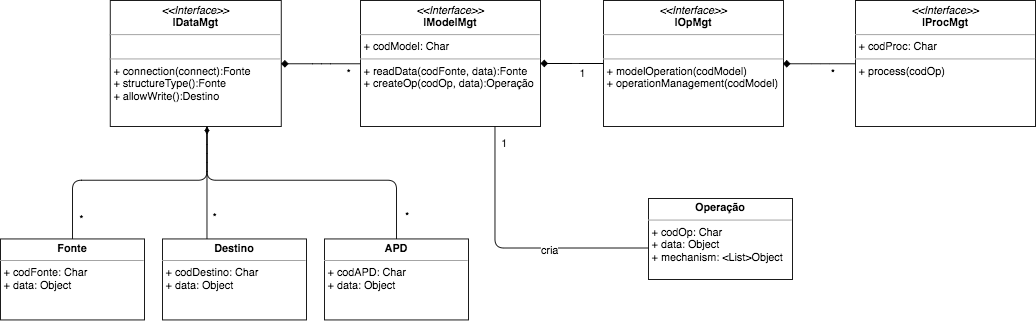
\includegraphics[scale=0.49]{fig/interfaces.png}
	\caption{Diagrama de especificação das interfaces de ETL4NoSQL}
	\label{interfaces}
\end{figure}


\section{Ambiente de Implementação}

Para a implementação do ETL4NoSQL utilizamos a linguagem de programação Python, pois ela segue o paradigma de orientação à objetos que é adequado para a proposta desta pesquisa. Além disso, Python tem uma sintaxe de fácil aprendizado e pode ser usada em diversas áreas, como Web e computação gráfica. Ela é uma linguagem de alto nível interpretada e também é um software livre. Devido a natureza do \textit{framework} ser flexível, reusável e integrado faz com que a orientação à objetos torne-se um bom paradigma a ser aproveitado neste trabalho.

Assim, a implementação do \textit{framework} foi baseada nos princípios do design orientado a objetos de inversão de controle, onde-se determina que os módulos de alto nível não devem ser dependentes de módulos de baixo nível, e sim, de abstrações, ou seja, os detalhes devem depender das abstrações. Esse princípio sugere que dois módulos não devem ser ligados diretamente, pois devem estar desacoplados com uma camada de abstração entre eles. Para suprir esse princípio, o ETL4NoSQL possui interfaces como o ETL4NoSQLMgr, IDataMgr, IModelMgr, IOpMgr e IProcMgr. Elas utilizam dos mesmos comportamentos para as diversas variações, porém aplicados de acordo com a especificidade de cada um. Outro princípio importante utilizado é o da segregação de interfaces onde os usuários não devem ser forçados a depender de interfaces que não necessitam, elas dever ser enxutas com métodos específicos para a interface. 

Na seção seguinte apresentaremos as interfaces de programação do ETL4NoSQL, como uma sugestão a ser utilizada para a implementação deste trabalho de dissertação.


\section{Interfaces de Programação}

O ETL4NoSQL possui cinco principais interfaces de programação (a arquitetura com as interfaces é apresentada na figura \ref{arquitetura}). O ETL4NoSQLMgr é a interface principal que interliga as demais interfaces, ela é a \textit{controller} (controlador) do \textit{framework}. Na figura \ref{etl4nosqlmgr} podemos ver a implementação da interface ETL4NoSQLMgr, nota-se que todas as outras quatro interfaces foram importadas nela. Nesta interface, também é realizada a execução dos processos de leitura e escrita das bases de dados fonte, destino e área de processamento de dados, cria a amostra dos dados a serem manipulados, as operações, realiza a execução das operações e as gerencia.

\begin{figure}[h!]
	\centering
	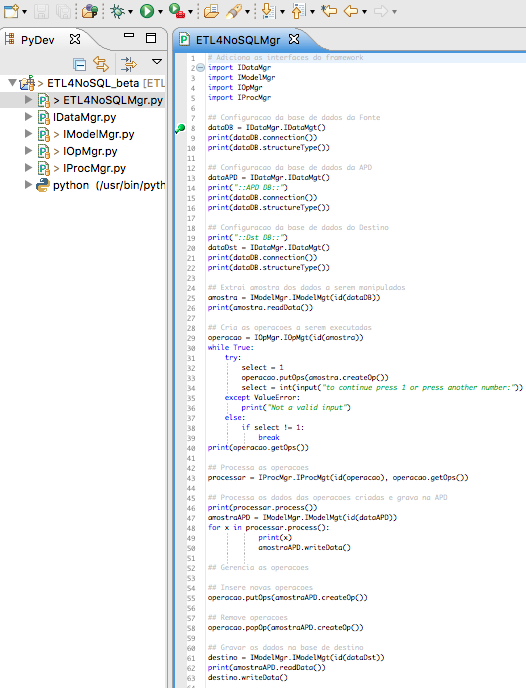
\includegraphics[scale=0.8]{fig/etl4nosqlmgr.png}
	\caption{Tela do IDE LiClipse com a implementação da interface ETL4NoSQLMgr}
	\label{etl4nosqlmgr}
\end{figure}

A interface IDataMgr pode ser vista na figura \ref{idatamgr}, ela é responsável pela conexão de todas as bases de dados, bem como determina o tipo de estrutura que é a base, e também, informa se há permissão para escrita na base de dados.

\begin{figure}[h!]
	\centering
	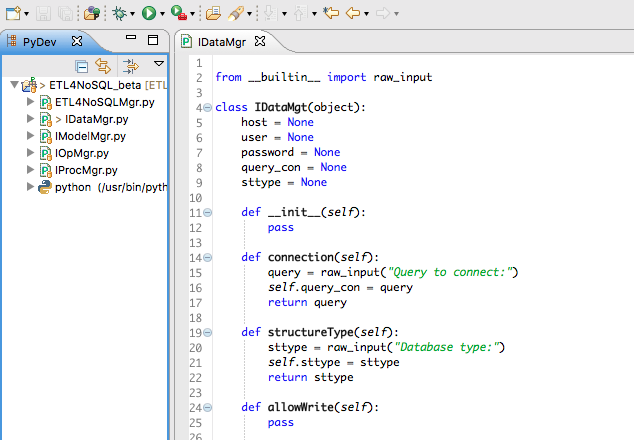
\includegraphics[scale=0.7]{fig/idatamgr.png}
	\caption{Tela do IDE LiClipse com a implementação da interface IDataMgr}
	\label{idatamgr}
\end{figure}

Na figura \ref{imodelmgr} é apresentada a interface IModelMgr, esta realiza a leitura dos dados da base determinada pela interface IDataMgr e configurada no controlador ETL4NoSQLMgr. A interface IModelMgr também cria as operações de ETL e grava os dados na base de dados determinada no controlador.

\begin{figure}[h!]
	\centering
	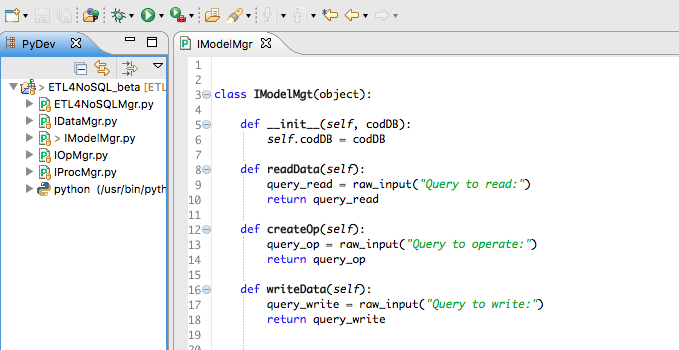
\includegraphics[scale=0.6]{fig/imodelmgr.png}
	\caption{Tela do IDE LiClipse com a implementação da interface IModelMgr}
	\label{imodelmgr}
\end{figure}

As operações criadas pela interface IModelMgr são listadas na interface IOpMgr (figura \ref{iopmgr}). Ela gerencia a inserção, alteração e remoção das operações, bem como ordena a sequência de operações a serem executadas.

\begin{figure}[h!]
	\centering
	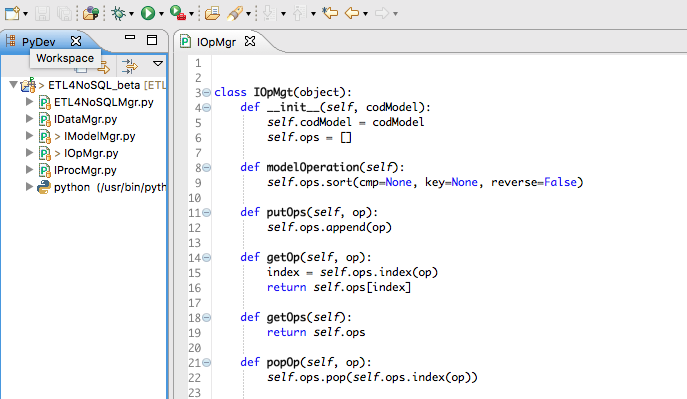
\includegraphics[scale=0.6]{fig/iopmgr.png}
	\caption{Tela do IDE LiClipse com a implementação da interface IOpMgr}
	\label{iopmgr}
\end{figure}

E finalmente, na figura \ref{iprocmgr}, é apresentada a interface IProcMgr. Esta interface é responsável pela execução das operações listadas pela IOpMgr. Na IProcMgr também é possível determinar o tipo de processamento desejável. 

\begin{figure}[h!]
	\centering
	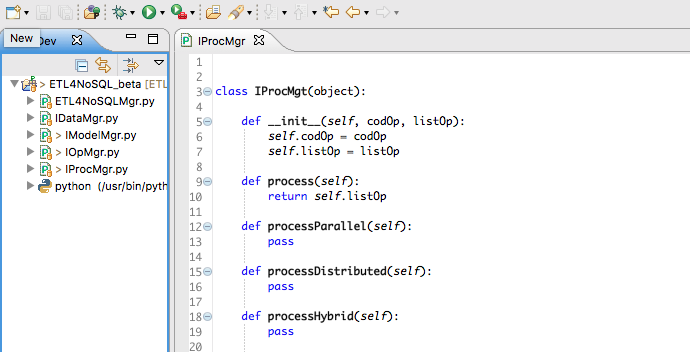
\includegraphics[scale=0.6]{fig/iprocmgr.png}
	\caption{Tela do IDE LiClipse com a implementação da interface IProcMgr}
	\label{iprocmgr}
\end{figure}

%De forma a detalhar a modelagem de especificação dos componentes deste trabalho, criamos um \textit{workflow} que é apresentado na figura \ref{modeloespecificacao} utilizando modelos informais e notações como a UML (\cite{clements:2002}).

%O modelo de processo do funcionamento da ferramenta ETL4NoSQL, baseado nas notações da UML 2.0 (\cite{clements:2002}), é representado na figura \ref{modeloprocesso}. Esse modelo descreve o processamento dos dados nas atividades de identificação dos dados, obtenção das informações para a importação e o mapeamento dos dados para os esquemas desejados, e também, a atividade dos processos de ETL para por fim dar carga dos dados em DWs, repositórios analíticos ou em arquivos XML.


% fluxo de processos da ferramenta ETL4NoSQL é o diagrama de atividades, que de acordo com a UML 2.0 tem como objetivo mostrar o fluxo de atividades em um único processo. O diagrama mostra como um atividade depende uma da outra. Na figura \ref{diagramaatividades} o diagrama mostra a interação dos componentes ao executar um processo de ETL, onde o estágio inicial é a importação dos dados seguido pelo mapeamento, após a obtenção dos dados necessários é possível a execução dos diversos processos de ETL em uma área de processamento para finalmente os dados serem exportados para base de destino.
%% utilizar diagrama de fluxo de dados para descrever os requisitos do sistema e diagrama de interações


%%construir um diagrama de atividades da execução de um processo de ETL



\section{Considerações Finais}

Este capítulo descreveu o ETL4NoSQL. Para isso, foram apresentados os requisitos de desenvolvimento de um \textit{framework} de ETL expondo a modelagem do domínio de ETL4NoSQL por meio de seu modelo conceitual, de casos de uso e comportamental. Foram demonstradas a modelagem da especificação, identificando os componentes, as interfaces de sistemas e de negócio do  \textit{framework} proposto. A especificação da arquitetura dos componentes do ETL4NoSQL e suas interações também foram evidenciadas. Mostramos como solução para implementação, as interfaces de programação utilizando a linguagem orientada à objetos chamada Python.

O capítulo seguinte apresentará um estudo experimental de \textit{software} que tem por objetivo avaliar se o ETL4NoSQL é um \textit{framework} adequado para modelar e executar operações de ETL em BDs NoSQL.


\chapter{Estudo Experimental de Software}

Este capítulo provê o roteiro de experimentação de software para ferramentas de ETL utilizando dados estruturados, semi estruturados e não estruturados. A Engenharia de Software Experimental tem como objetivo aprimorar métodos, técnicas e ferramentas de Engenharia de Software a partir de métodos experimentais (Isaque Elcio de Souza, TESE - Um sistema de Inf para Geren de Projetos Experimentais em ES). As etapas definidas no processo de experimentação em Engenharia de Software proposto por [Amaral (),Isaque Elcio de Souza, TESE ] consiste em etapas de definição, planejamento, operação, interpretação dos dados e empacotamento que serão melhor detalhados nas seções a seguir.
\clearpage

\section{Objetivos do experimento}

O objetivo principal da aplicação deste experimento é definir se o framework proposto por esta pesquisa de dissertação é uma ferramenta adequada para auxiliar no desenvolvimento de processos de ETL em dados estruturados, semi estruturados e não estruturados.

\subsection{Objetivo da Medição}

Tendo como base as ferramentas de ETL existentes na literatura, caracterizar:

\begin{enumerate}
	\item Quais as principais funcionalidades que as ferramentas de ETL oferecem:
	\begin{enumerate}
		\item essas funcionalidades manipulam dados estruturados, semi estruturados e não estruturados.
		\item  essas funcionalidades não manipulam dados estruturados, semi estruturados e não estruturados.
	\end{enumerate}
	\item Quais funcionalidades podem ser consideradas fundamentais para a produtividade na criação de processos de ETL:
	\begin{enumerate}
		\item quais necessitam manipular dados em grande escala.
		\item quais não manipulam grande volume de dados.
	\end{enumerate}
	\item Quais funcionalidades poderiam aprimorar as ferramentas de ETL.
\end{enumerate}

\subsection{Objetivos do Estudo}

\begin{itemize}
	\item Analisar as ferramentas de ETL para dados estruturados, semi estruturados e não estruturados;
	
	\item Com o propósito de caracterizar;
	
	\item Com respeito à intersecção das ferramentas de ETL existente;
	
	\item Do ponto de vista da literatura;
	
	\item No contexto de comparativo entre as ferramentas mais conhecidas no mercado atual.
\end{itemize}


\subsection{Questões}

Q1. Existem funcionalidades listadas pelas ferramentas pesquisadas que não estão presentes no ETL4NoSQL?

Métrica: A lista de funcionalidades que não estão presentes no ETL4NoSQL.

Q2. Existem funcionalidades oferecidas pelo ETL4NoSQL que não estão presentes nas ferramentas apresentadas pela literatura?

Métrica: A lista de funcionalidades que não estão presentes nas ferramentas da literatura.

Q3. Existem funcionalidades que não estão presentes no ETL4NoSQL e nas ferramentas da literatura que poderiam ser implementadas?

Métrica: A lista de funcionalidades que não estão presentes em nenhuma das ferramentas.

\section{Planejamento}

Na etapa de planejamento são definidas as hipóteses do estudo, a descrição da instrumentação, as métricas, seleção do contexto e dos indivíduos, as variáveis, a análise qualitativa e a validade do experimento. Todas elas serão descritas nas seções seguintes.

\subsection{Definição das Hipóteses}

Hipótese nula (H0): As funcionalidades oferecidas pelo ETL4NoSQL são similares às funcionalidades oferecidas pelas ferramentas presentes na literatura.

Fp - Funcionalidades do ETL4NoSQL

Fl - Funcionalidades das ferramentas da literatura

H0: Fl - (Fp $\cap$ Fl) = $\emptyset$
\newline

Hipótese alternativa (H1): A lista de funcionalidades oferecidas pelo ETL4NoSQL é diferente da lista de funcionalidades oferecidas pelas ferramentas presentes na literatura.

Fp - Funcionalidades do ETL4NoSQL

Fl - Funcionalidades das ferramentas da literatura

H1: Fl - (Fp $\cap$ Fl) $\neq$ $\emptyset$
\newline

Hipótese alternativa (H2): A lista de funcionalidades que poderiam ser implementadas é diferente da lista de funcionalidades oferecidas pelas ferramentas na literatura e pelo ETL4NoSQL.

Fp - Funcionalidades do ETL4NoSQL

Fl - Funcionalidades das ferramentas da literatura

Fi - Funcionalidades que poderiam ser implementadas

H2: Fi - (Fp $\cap$ Fl $\cap$ Fi) $\neq$ $\emptyset$

\subsection{Descrição da instrumentação}

Para cada funcionalidade presente nas ferramentas apresentada na literatura que são consideradas fundamentais para o funcionamento dos processos de ETL pode ser encontrada no quadro \ref{instrumentacao}:

\begin{table}[ht]
	\centering
	\caption{Descrição da Instrumentação}
	\label{instrumentacao}
	\begin{tabular}{|p{5cm}| p{5cm} | p{5cm}|}
		\hline
		Presença da Funcionalidade (P) & Melhoria da Funcionalidade (M) & Utilidade da Funcionalidade (U)\\
		\hline
		\begin{enumerate}
			\item Não está presente
			\item Está presente parcialmente
			\item Está presente
		\end{enumerate} & 
		\begin{enumerate}
			\item Necessita melhorar
			\item Não há necessidade de melhoria
			\item Pode melhorar, mas não necessidade
		\end{enumerate} &
		\begin{enumerate}
			\item É útil
			\item Não é útil
			\item É parcialmente útil
		\end{enumerate}\\
		\hline
		
	\end{tabular}
\end{table}

Para cada funcionalidade aplicar teste estatístico Chi-2 para definir:

se pode considerar que essa funcionalidade é fornecida;

se pode considerar que essa funcionalidade é útil;

se pode considerar que essa funcionalidade necessita de melhoria.

Resultado: N funcionalidades com valores (P; M; U) onde P - presença {0 - não presente; 1 - presente}; U - utilidade {0 - não é útil; 1 - é útil}; melhoria {0 - não necessita melhorar; 1 - necessita melhorar}.

\subsection{Métricas}

Na tabela \ref{metricas} são apresentadas as métricas utilizadas neste experimento.

\begin{table}[ht!]
	\centering
	\caption{Métricas}
	\label{metricas}
	\begin{tabular}{|p{0.5cm}| p{0.5cm} | p{0.5cm}| p{0.5cm}|p{9cm}|p{3cm}|}
		\hline
		N$\circ$ & P & M & U & Descrição da Funcionalidade & Questões\\
		\hline
		1 & 0 & 0 & 0 & Não está presente, não necessita melhorar, não é útil & N/A\\
		\hline
		2 & 0 & 0 & 1 & Não está presente, não necessita melhorar, é útil & Q3\\
		\hline
		3 & 0 & 1 & 0 & Não está presente, necessita melhorar, não é útil & N/A\\
		\hline
		4 & 0 & 1 & 1 & Não está presente, necessita melhorar, é útil & Q3\\
		\hline
		5 & 1 & 0 & 0 & Está presente, não necessita melhorar, não é útil & Q1, Q2\\
		\hline
		6 & 1 & 0 & 1 & Está presente, não necessita melhorar, é útil & Q1, Q2\\
		\hline
		7 & 1 & 1 & 0 & Está presente, necessita melhorar, não é útil & Q1, Q2\\
		\hline
		8 & 1 & 1 & 1 & Está presente, necessita melhorar, é útil & Q1, Q2\\
		\hline
		
		
		
	\end{tabular}
\end{table}	

\subsection{Seleção do contexto}

De acordo com Travassos (2002), o contexto pode ser caracterizado conforme quatro dimensões:

\begin{itemize}
	\item o processo: on-line / off-line;
	\item os participantes: ferramentas de ETL;
	\item realidade: o problema real / modelado;
	\item generalidade: específico / geral.
\end{itemize}

Nosso estudo supõe o processo off-line porque as ferramentas não estão sendo testadas durante todo o tempo da utilização, mas em certo instante. Os participantes são as ferramentas de ETL encontradas na literatura. O estudo é modelado porque as funcionalidades das ferramentas não são caracterizadas durante a resolução do problema real, mas utilizando parâmetros subjetivos (ex. presença, utilidade e necessidade). As funcionalidades do ETL4NoSQL são comparadas com as ferramentas presentes na literatura, então, o contexto possui o caráter específico.

\subsection{Seleção dos indivíduos}

Como participantes para o estudo propõe-se utilizar as ferramentas encontradas na literatura. Assume-se que esses indivíduos estão presente em diversos estudos realizados e avaliados no meio acadêmico.

Para a escolha das ferramentas utilizadas neste estudo foi levado em consideração a semelhança da finalidade do uso com a ferramenta proposta. Seria conveniente utilizar para o estudo ferramentas que tem o objetivo de auxiliar processos de ETL em diversas estruturas de dados. Dessa forma, a seleção baseou-se nas características das ferramentas.

\subsection{Variáveis}


Variável independente: A lista de funcionalidades das ferramentas encontradas na literatura.

Variáveis dependentes: 

\begin{enumerate}
	\item A similaridade entre as funcionalidades oferecidas pela ferramenta proposta e as funcionalidades encontradas nas ferramentas da literatura.
	
	Pode receber os valores: Igual, quando todas as funcionalidades tem o valor PMU = \{ 1, X, X \} (métricas 5-8);
	Diferente, quando todas as funcionalidades tem o valor PMU = \{ 0, X, X \} (métricas 1-4)
	Similar, quando não se cumprem as condições de "Igual" e "Diferente". O grau de similaridade pode ser avaliado como:
	\{ 1, X, X \} / \{ 0, X, X \} + \{ 1, X, X \} * 100\%
	
	\item A utilidade das funcionalidades similares. Mostra a parte útil das funcionalidades oferecidas pela ferramenta proposta:
	Parte útil: \{ 1, X, 1 \} / \{ 1, X, X \} * 100\%
	Parte inútil: \{ 1, X, 0 \} / \{ 1, X, X \} * 100\%
	
	\item A melhoria das funcionalidades similares. Mostra a necessidade de melhoria nas funcionalidades oferecidas pela ferramenta proposta:
	Não necessita melhorar: \{ 1, 0, X \} / \{ 1, X, X \} * 100\%
	Necessita melhorar: \{ 1, 0, X \} / \{ 1, X, X \} * 100\%
\end{enumerate}

\subsection{Análise Qualitativa}

Para analisar a informação referente às funcionalidades não oferecidas no ETL4NoSQL, mas que poderiam ser implementadas, propõe-se aplicar a análise qualitativa. Essa análise deve apresentar a lista de funcionalidades presentes nas ferramentas da literatura, que não estão presentes na ferramenta proposta, mas que são consideradas necessárias para facilitar a manipulação de dados estruturados, semi estruturados e não estruturados.
Assim, essa análise deve considerar funcionalidades com valor PMU = {0, X, X} (métricas 1-4) e a opção ''É útil'' para ''utilidade da funcionalidade''.

\subsection{Validade}

\textbf{Validade interna:} como mencionado na parte "Seleção dos indivíduos" para o estudo se propõe a utilizar ferramentas presentes na literatura, que são validadas pelo meio acadêmico. Assim, assume-se que elas são representativas para a população de ferramentas de ETL.

Além disso, para redução da influência dos fatores que não são interesse do nosso estudo e, portanto, para aumento da validade interna do estudo supõe-se utilizar dados das ferramentas mais populares da literatura, cuja a validação já tenha passado por diversas avaliações.

\textbf{Validade de conclusão:} para receber os valores da presença, utilidade e melhorias o teste binomial será utilizado. A verificação de hipótese será feita por meio de simples demonstração de presença ou não de funcionalidades nas listas que representam as variáveis independentes.

\textbf{Validade de construção:} esse estudo está caracterizado pela conformidade das funcionalidades listadas na ferramenta proposta com as funcionalidades reais necessárias para a utilização de ferramentas de ETL. As características das ferramentas de ETL presentes na literatura representa a lista de funcionalidades que uma ferramenta de ETL deve apresentar para mostrar o desempenho adequado do ponto de vista da literatura. As funcionalidades, que tem o maior relacionamento com as ferramentas de ETL do ponto de vista dos pesquisadores, foram escolhidas do conjunto total de funcionalidades das ferramentas de ETL presentes na literatura.

\textbf{Validade externa:} como foi mencionado nas partes "Seleção dos indivíduos" e "Validade interna" os participantes do estudo em geral podem ser considerados representativos para a população da literatura apresentada pela academia. Para avaliação do nível de importância das funcionalidades analisadas foi levada em consideração a frequência que a funcionalidade apareceu nas ferramentas da literatura.

Os materiais utilizados no estudo podem ser considerados representativos e "em tempo" para o problema sob análise, porque se compõem das funcionalidades de ferramentas de ETL presentes na literatura atual.

\section{Operação}

A etapa de operação ocorre após a etapa de planejamento do estudo experimental. Nela é exercido o monitoramento do experimento para garantir que ele esteja ocorrendo conforme foi planejado (Souza Isaque, 2015). Nesta seção serão apresentados os questionários do perfil da ferramenta de ETL e o de Funcionalidades.

\subsection{Questionário do Perfil da Ferramenta de ETL}

O quadro \ref{questionarioperfil} mostra as questões usadas para definir o perfil das ferramentas utilizadas como indivíduos deste experimento.

\begin{table}[ht]
	\centering
	\caption{Questionário do Perfil da Ferramenta de ETL}
	\label{questionarioperfil}
	\begin{tabular}{|p{8cm}| p{8cm}| }
		\hline
		Nome da ferramenta de ETL: & \\
		\hline
		Possui código aberto? & Sim $\bigcirc$ Não $\bigcirc$ \\
		\hline
		Possui uma marca reconhecida no mercado? & Sim $\bigcirc$ Não $\bigcirc$ \\
		\hline
		Tem como finalidade utilizar bancos de dados NoSQL? &  Sim $\bigcirc$ Não $\bigcirc$ \\
		\hline
		Possui interface gráfica? & Sim $\bigcirc$ Não $\bigcirc$ \\
		\hline
		É programável?  & Sim $\bigcirc$ Não $\bigcirc$ \\
		\hline
		É integrada? & Sim $\bigcirc$ Não $\bigcirc$ \\
		\hline
		Qual o tipo de processamento que a ferramenta executa? & Distribuído  $\bigcirc$  Centralizada  $\bigcirc$  Híbrido  $\bigcirc$ \\
		\hline
		É extensível? & Sim $\bigcirc$ Não $\bigcirc$ \\
		\hline
		Para qual finalidade a ferramenta procura auxiliar melhor os processos de ETL? & Modelagem $\bigcirc$ Desempenho $\bigcirc$ Ambos $\bigcirc$ \\
		\hline
		
		
	\end{tabular}
\end{table}


\subsection{Questionário de Funcionalidades}

Sob o ponto de vista das características das ferramentas e considerando a finalidade da ferramenta indicada acima, avalie as colunas correspondentes segundo as escalas abaixo, a presença, utilidade e melhorias quanto às funcionalidades das ferramentas apresentadas nos seus respectivos trabalhos de pesquisa, das funcionalidades listadas no questionário:

\begin{table}[ht!]
	\centering
	\caption{Instrumentação para aplicar o questionário}
	\label{instrumentacao2}
	\begin{tabular}{|p{5cm}| p{5cm} | p{5cm}|}
		\hline
		Presença da Funcionalidade (P) & Melhoria da Funcionalidade (M) & Utilidade da Funcionalidade (U)\\
		\hline
		\begin{enumerate}
			\item Não está presente
			\item Está presente parcialmente
			\item Está presente
		\end{enumerate} & 
		\begin{enumerate}
			\item Necessita melhorar
			\item Não há necessidade de melhoria
			\item Pode melhorar, mas não necessidade
		\end{enumerate} &
		\begin{enumerate}
			\item É útil
			\item Não é útil
			\item É parcialmente útil
		\end{enumerate}\\
		\hline
		
	\end{tabular}
\end{table}

\begin{figure}[h!]
	\centering
	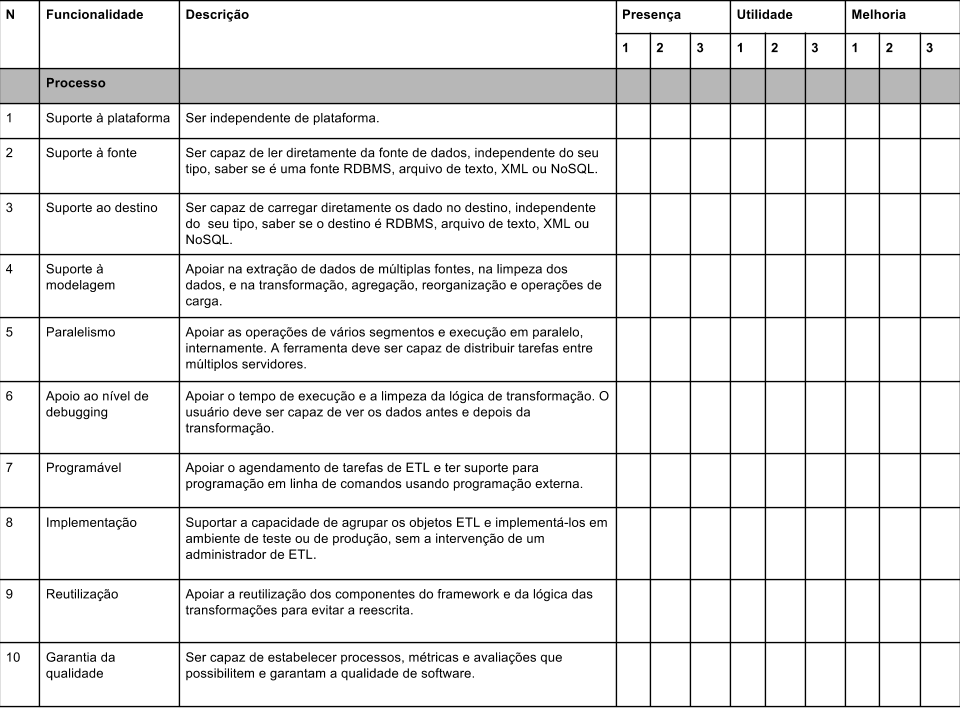
\includegraphics[scale=0.5]{fig/questionario_caracteristicas.png}
	\caption{Questionário de Funcionalidades}
	\label{questionariofuncionalidades}
\end{figure}

\clearpage

\subsection{Resultado do Estudo}


A figura \ref{presenca} apresenta o gráfico da quantidade de presença para cada funcionalidade de acordo com cada ferramenta de ETL. Já a figura \ref{utilidade} mostra o nível de importância que as ferramentas dão para cada funcionalidade e a figura \ref{melhoria} indica necessidade de melhorar funcionalidade em cada ferramenta.

\begin{figure}[h]
	\centering
	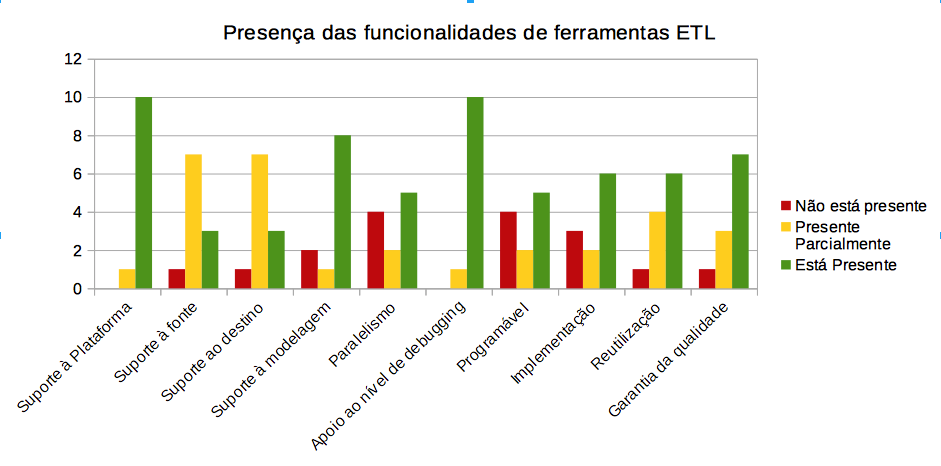
\includegraphics[scale=0.5]{fig/presenca.png}
	\caption{Quantidade de Presença para cada funcionalidade}
	\label{presenca}
\end{figure}

\begin{figure}[h]
	\centering
	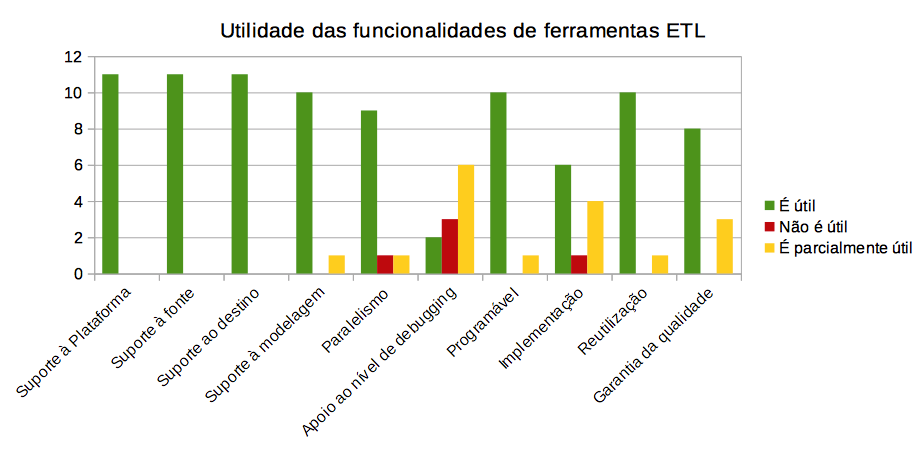
\includegraphics[scale=0.5]{fig/utilidade.png}
	\caption{Níveis de utilidade para cada funcionalidade}
	\label{utilidade}
\end{figure}

\begin{figure}[h]
	\centering
	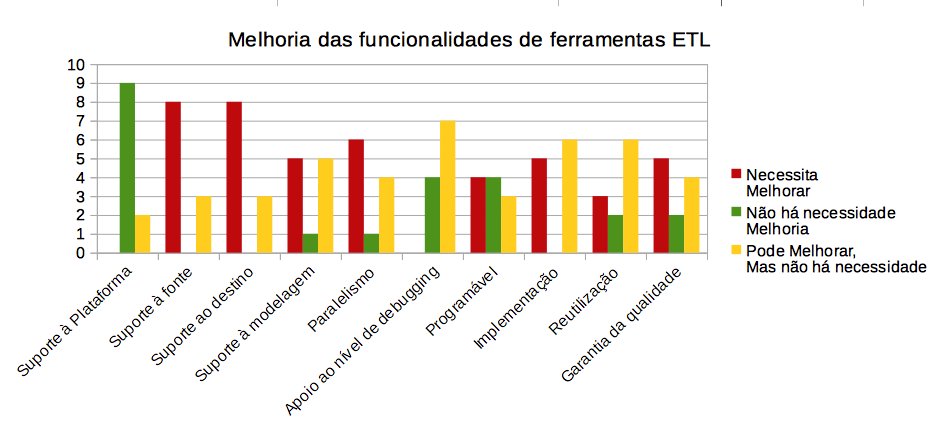
\includegraphics[scale=0.5]{fig/melhorias.png}
	\caption{Necessidade de melhoria para cada funcionalidade}
	\label{melhoria}
\end{figure}

\clearpage

O perfil dos participantes é apresentado no quadro \ref{resultadoperfil}, bem como a legenda para leitura do resultado.

\begin{table}
	\centering
	\caption{Resultado do Perfil dos participantes}
	\label{resultadoperfil}
\resizebox{\textwidth}{!}{\begin{tabular}{|r|r|r|r|r|r|r|r|r|r|}
		\hline
		Ferramenta & Código Fonte & Marca de mercado & Para NoSQL & GUI & Programável & Integrada & Processamento & Extensível & Finalidade\\
		\hline
		PygramETL  & 1 & 2 & 2 & 2 & 1 & 1 & 2 & 1 & 2 \\
		\hline
		
		
		
	\end{tabular}}
\end{table}
% ---
\section{Descrição}
\section{Considerações Finais}

\chapter{Conclusão}


A existência de uma demanda crescente para integrar os dados modelados em vários tipos de estruturas em um repositório unificado, além de muitas empresas encontrarem dificuldades para lidar com as ferramentas ETL disponíveis no mercado motivaram esta pesquisa, cuja apresentou o ETL4NoSQL. Este capítulo resume o trabalho exposto nesta dissertação apresentando suas contribuições relevantes, seus desafios e dificuldades, seus resultados e trabalhos futuros a partir do ETL4NoSQL. 


Portanto, este trabalho propôs um \textit{framework} programável para desenvolvimento de aplicações de ETL que possibilita a extração, transformação e carga de dados armazenados em BDs NoSQL. O \textit{framework} possui um ambiente integrado para a leitura e escrita dos dados, além da modelagem e execução distribuída ou centralizada dos processos de ETL. O componente de gerenciamento de dados do \textit{framework} executa os processos de ETL em BDs NoSQL. Esse componente possibilita a leitura e manipulação de dados em BDs NoSQL, e também o armazenamento desses dados em bases deste tipo, oferecendo uma alternativa de modelo não relacional para a construção de DWs.

\clearpage

\section{Principais Contribuições}

Uma das principais contribuições do nosso trabalho é o \textit{framework} ETL4NoSQL, que engloba os requisitos de \textit{software} para ferramentas de ETL, a modelagem do domínio, através de seus três modelos: modelo conceitual, de casos de uso e de comportamento; a modelagem da especificação, da arquitetura e especificação dos componentes, identificação das interfaces de sistemas e de negócio, bem como a interação entre os componentes do ETL4NoSQL. O ETL4NoSQL pode ser utilizado para o desenvolvimento de novas aplicações de ETL. As especificações de seus componentes podem ser reutilizados para facilitar a especialização e instanciação de novas aplicações de ETL.

Outra contribuição deste trabalho é o estudo experimental de \textit{software} baseado nas ferramentas de ETL encontradas na literatura por esta pesquisa. O estudo teve como objetivo definir se o ETL4NoSQL é adequado para auxiliar no desenvolvimento de processos de ETL. Os resultados do estudo mostraram que o ETL4NoSQL possui um grau de similaridade de 70\% em relação com as outras 11 ferramentas estudadas nesta pesquisa, e que dessa similaridade 85,71\% das funcionalidades são consideradas úteis para desenvolver processos de ETL.

Dessa forma, podemos concluir que o objetivo da presente proposta, de especificar um \textit{framework} programável, flexível e integrado para extração, transformação e carga dos dados em BDs NoSQL foi atingido de forma efetiva e satisfatória, no sentido de facilitar e flexibilizar a atividade de desenvolvimento de novas ferramentas de ETL.

\section{Discussão}

Na seção 2.2 apresentamos os trabalhos correlatos a esta pesquisa, nesta seção foi demonstrada as ferramentas de ETL mais citadas pela literatura. Podemos observar que a maioria das ferramentas pesquisadas foca no desempenho ao lidar com grandes volumes de dados e BDs NoSQL, porém nenhuma delas apresentou uma solução alternativa para modelagem de BDs NoSQL ficando a cargo do desenvolvedor encontrar meios para esquematizar os dados. Algumas delas, como a P-ETL, oferece alternativas para leituras de arquivos textuais, mas não dão enfoque aos BDs NoSQL.  Outras ferramentas como o ETLMR, CloudETL e BigETL utilizam processamento paralelo e distribuído para facilitar a execução de processos de ETL em grandes volumes de dados, contudo não lidam com a modelagem e leitura dos dados não relacionais.

Assim, como alternativa a isso, sugerimos o ETL4NoSQL que consiste em um \textit{framework} baseado em componentes, programável, flexível e integrado. Os seus componentes podem ser reutilizados, por meio de suas interfaces e especializados para atender as especificidades de cada demanda.


\section{Trabalhos Futuros}

Como trabalhos futuros indicamos a execução de testes com dados reais. Adicionalmente, testar o desempenho com a execução dos processos de forma distribuída, centralizada e paralela. E finalmente, verificar a eficiência comparada aos outros métodos existentes para o desenvolvimento de aplicações de ETL.




% References

\begin{references}
  \bibliography{references}
\end{references}

% Appendix

\theappendix
\chapter{Fichas de Respostas ao questionário de funcionalidades das ferramentas de ETL}
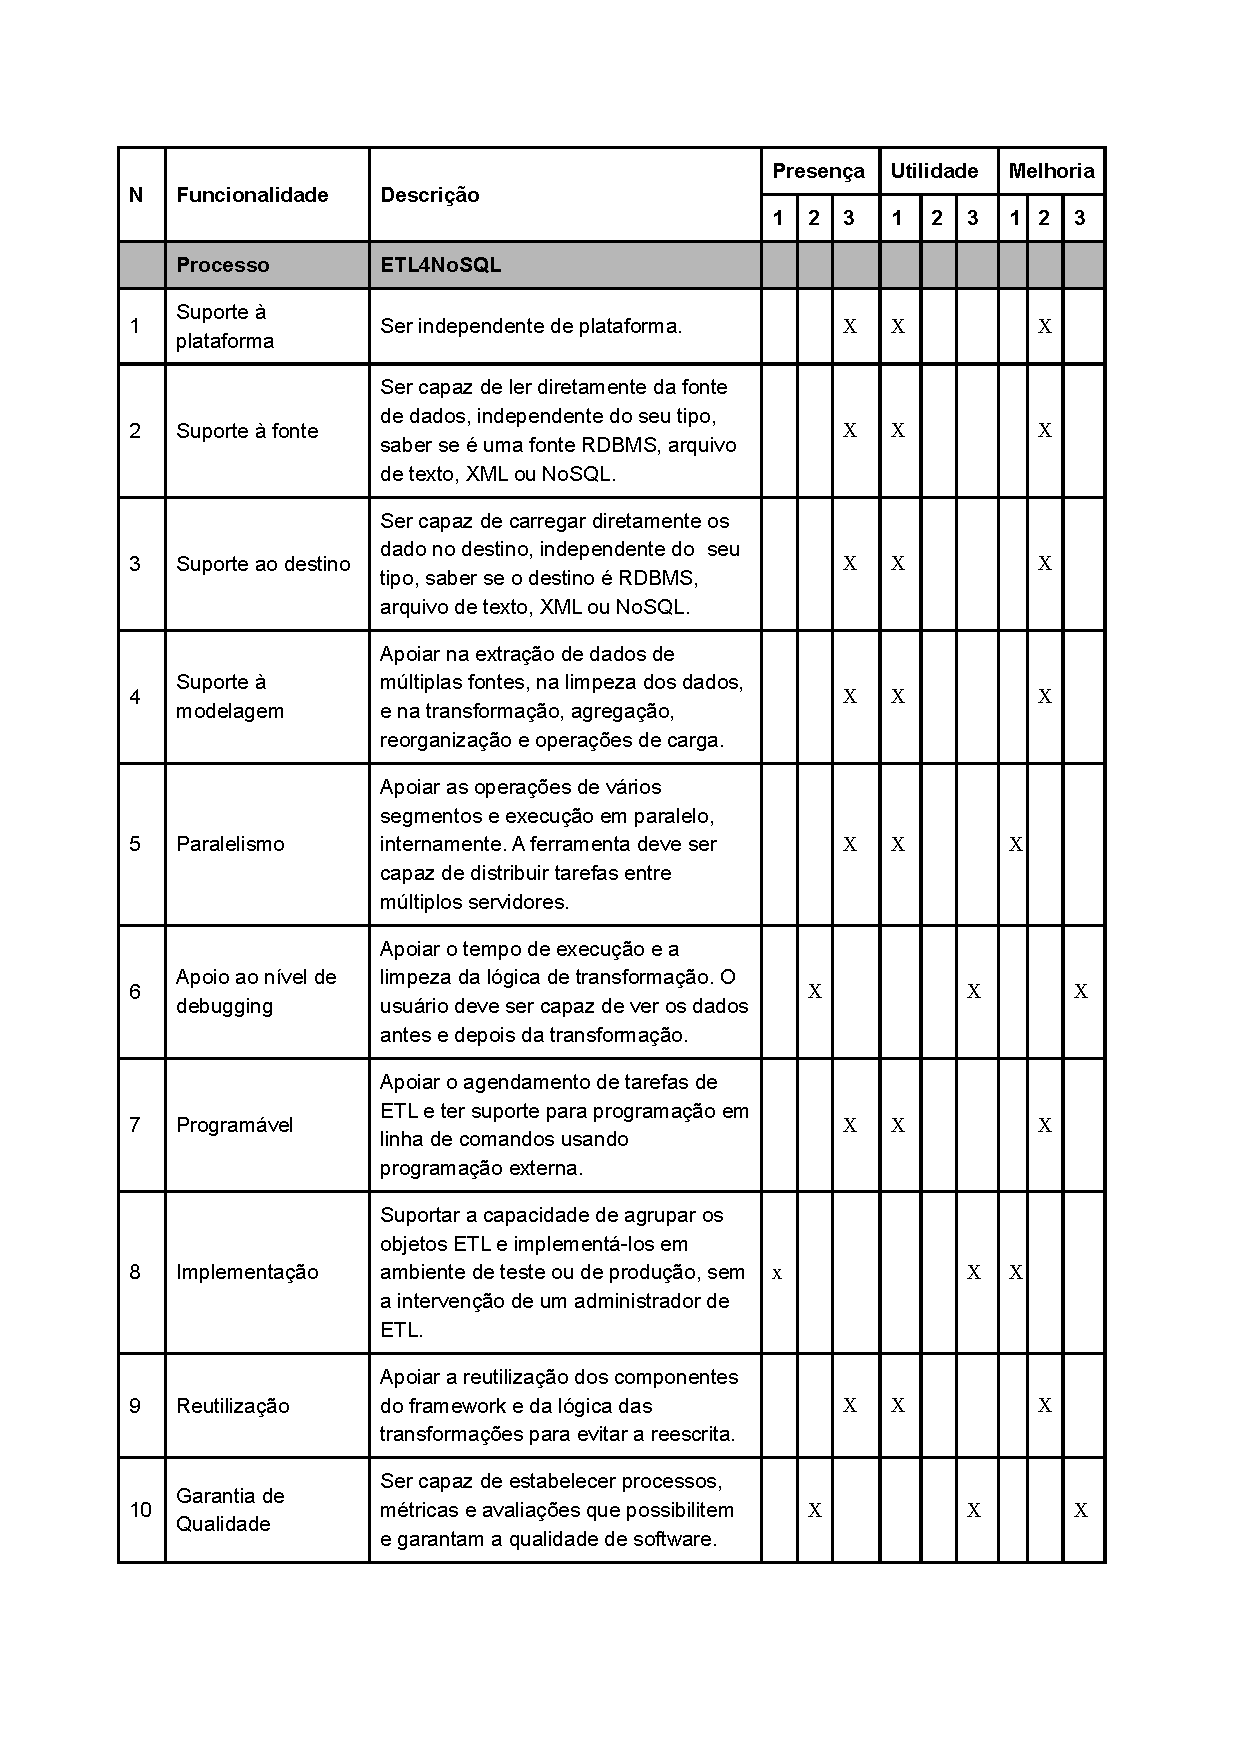
\includepdf[pages=1-12]{appendix/fichasquestionario.pdf} % incluirá o arquivo todo

\chapter{Planilha de Características das Ferramentas de ETL}
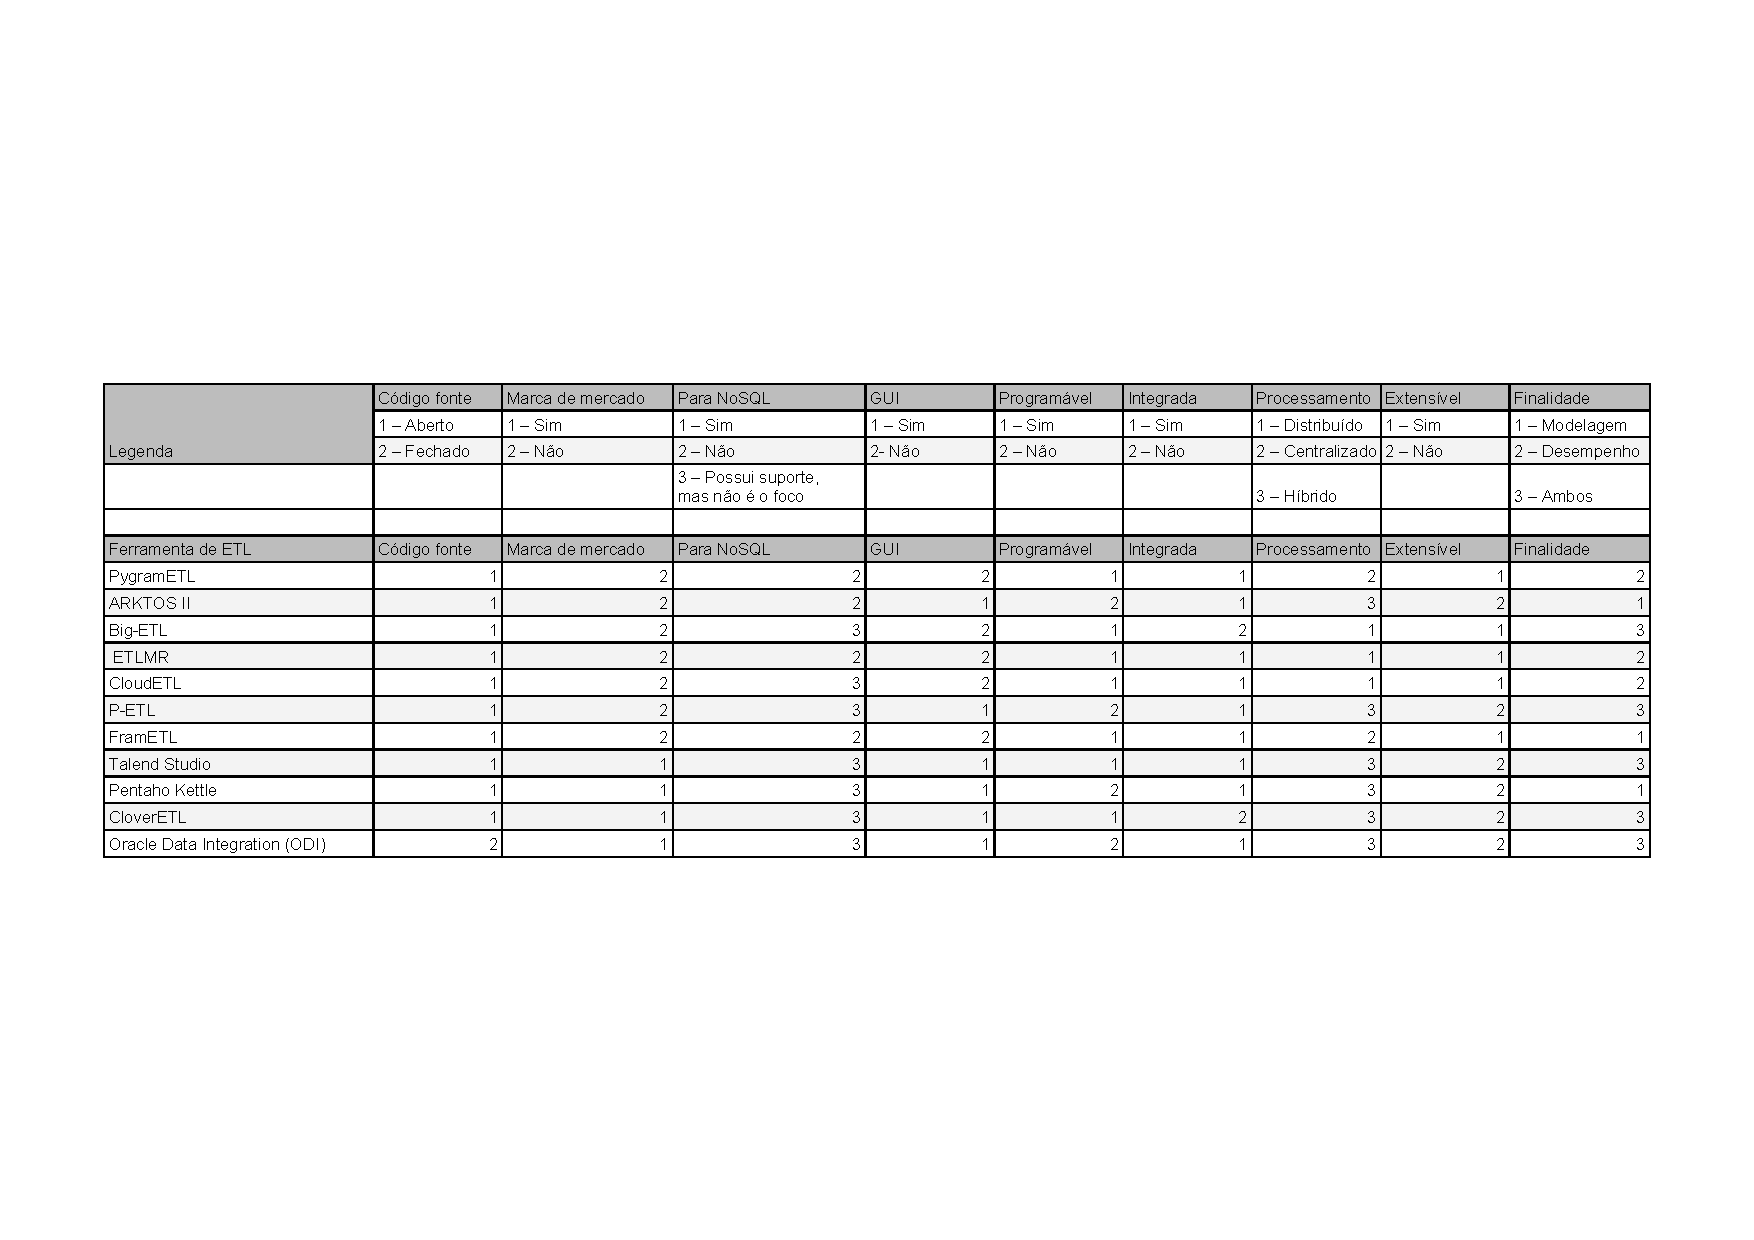
\includepdf[landscape]{appendix/fichacaracteristicas.pdf}

\end{document}
